% Author Name: José Areia 
% Author Contact: jose.apareia@gmail.com
% Version: 2.2.5 - 2025/04/16
% Public Repository: https://github.com/joseareia/ipleiria-thesis
% Wiki/Getting Help: https://github.com/joseareia/ipleiria-thesis/wiki

%%% Document Options %%%
\documentclass[
    language=spanish,
    school=estg,
    docstage=final,
    media=paper,
    linkcolor=red!45!black,
    chapterstyle=classic,
    coverstyle=classic
]{IPLeiriaThesis} % Refer to the Wiki for a list of available options.

%%% Document Version %%%
\DocumentVersion{1.0.0} % This is required only if the 'docstage' is set to 'working'.

%%% Document Metadata %%%
% First Author (Mandatory)
\FirstAuthor{Over Haider Castrillón Valencia}
\FirstAuthorNumber{2230455}

% Second Author (Optional)
% \SecondAuthor{Jane Smith}
% \SecondAuthorNumber{2230456}

% Third Author (Optional)
% \ThirdAuthor{July Smith}
% \ThirdAuthorNumber{2230457}

% % Supervisor (Mandatory)
\Supervisor{Gustavo Isaza Echeverry}
% \SupervisorMail{joe.smith@ipleiria.pt}
% Please provide: [Current Title, Affiliation]
% \SupervisorTitle{Gustavo Adolfo Echeverry Isaza, Universidad de Caldas} 

% Co-Supervisor (Optional)
% \CoSupervisor{Steve Smith}
% \CoSupervisorMail{steve.smith@ipleiria.pt}
% \CoSupervisorTitle{Associate Professor, Polytechnic of Leiria}

% Second Co-Supervisor (Optional)
% \SecCoSupervisor{Shak Smith}
% \SecCoSupervisorMail{shak.smith@ipleiria.pt}
% \SecCoSupervisorTitle{Associate Researcher, Computer Science \& Communication Research Centre}

% Title (Mandatory)
\Title{Segundo Parcial}

% Subtitle (Mandatory)
\Subtitle{Ciberseguridad\\Segundo parcial}

% University (Mandatory)
\University{Universidad de Caldas}

% % School (Mandatory)
\School{Facultad de Inteligencia Artificial e Ingenierías}

% Department (Mandatory)
\Department{Facultad de Inteligencia Artificial e Ingenierías}

% Degree (Mandatory)
\Degree{Ingeniería en Sistemas y Computación}

% Course (Optional)
% \Course{Offensive \& Defensive Cybersecurity}

% Thesis Theme (Mandatory)
\ThesisType{Dissertation/Project/Internship \\ \textcolor{blue}{(Erase the Non-Essential)}}

% Local & Date (Mandatory)
\Date{Manizales Caldas, \DTMmonthname{\month}~\number\day~de~\number\year}

% Academic Year 
\AcademicYear{2024/25}

%%% Loading of Glossary and Acronyms %%%
\makeglossaries
\loadglsentries{Matter/04-Glossary}
\loadglsentries[\acronymtype]{Matter/05-Acronyms}

\begin{document}

%%% Front Matter %%%
\ifthenelse{\equal{\CoverOption}{classic}}{
    \newcommand\BackgroundPicCover{%
    \put(0,0){%
    \parbox[b][\paperheight]{\paperwidth}{%
    \vfill
    \centering
    
\includegraphics[width=\paperwidth,height=\paperheight,keepaspectratio]{Figures/Theme/Cover-BG.pdf}%
    \vfill
    }}}
}{
    \newcommand\BackgroundPicCover{%
    \put(0,0){%
    \parbox[b][\paperheight]{\paperwidth}{%
    \vfill
    \centering
    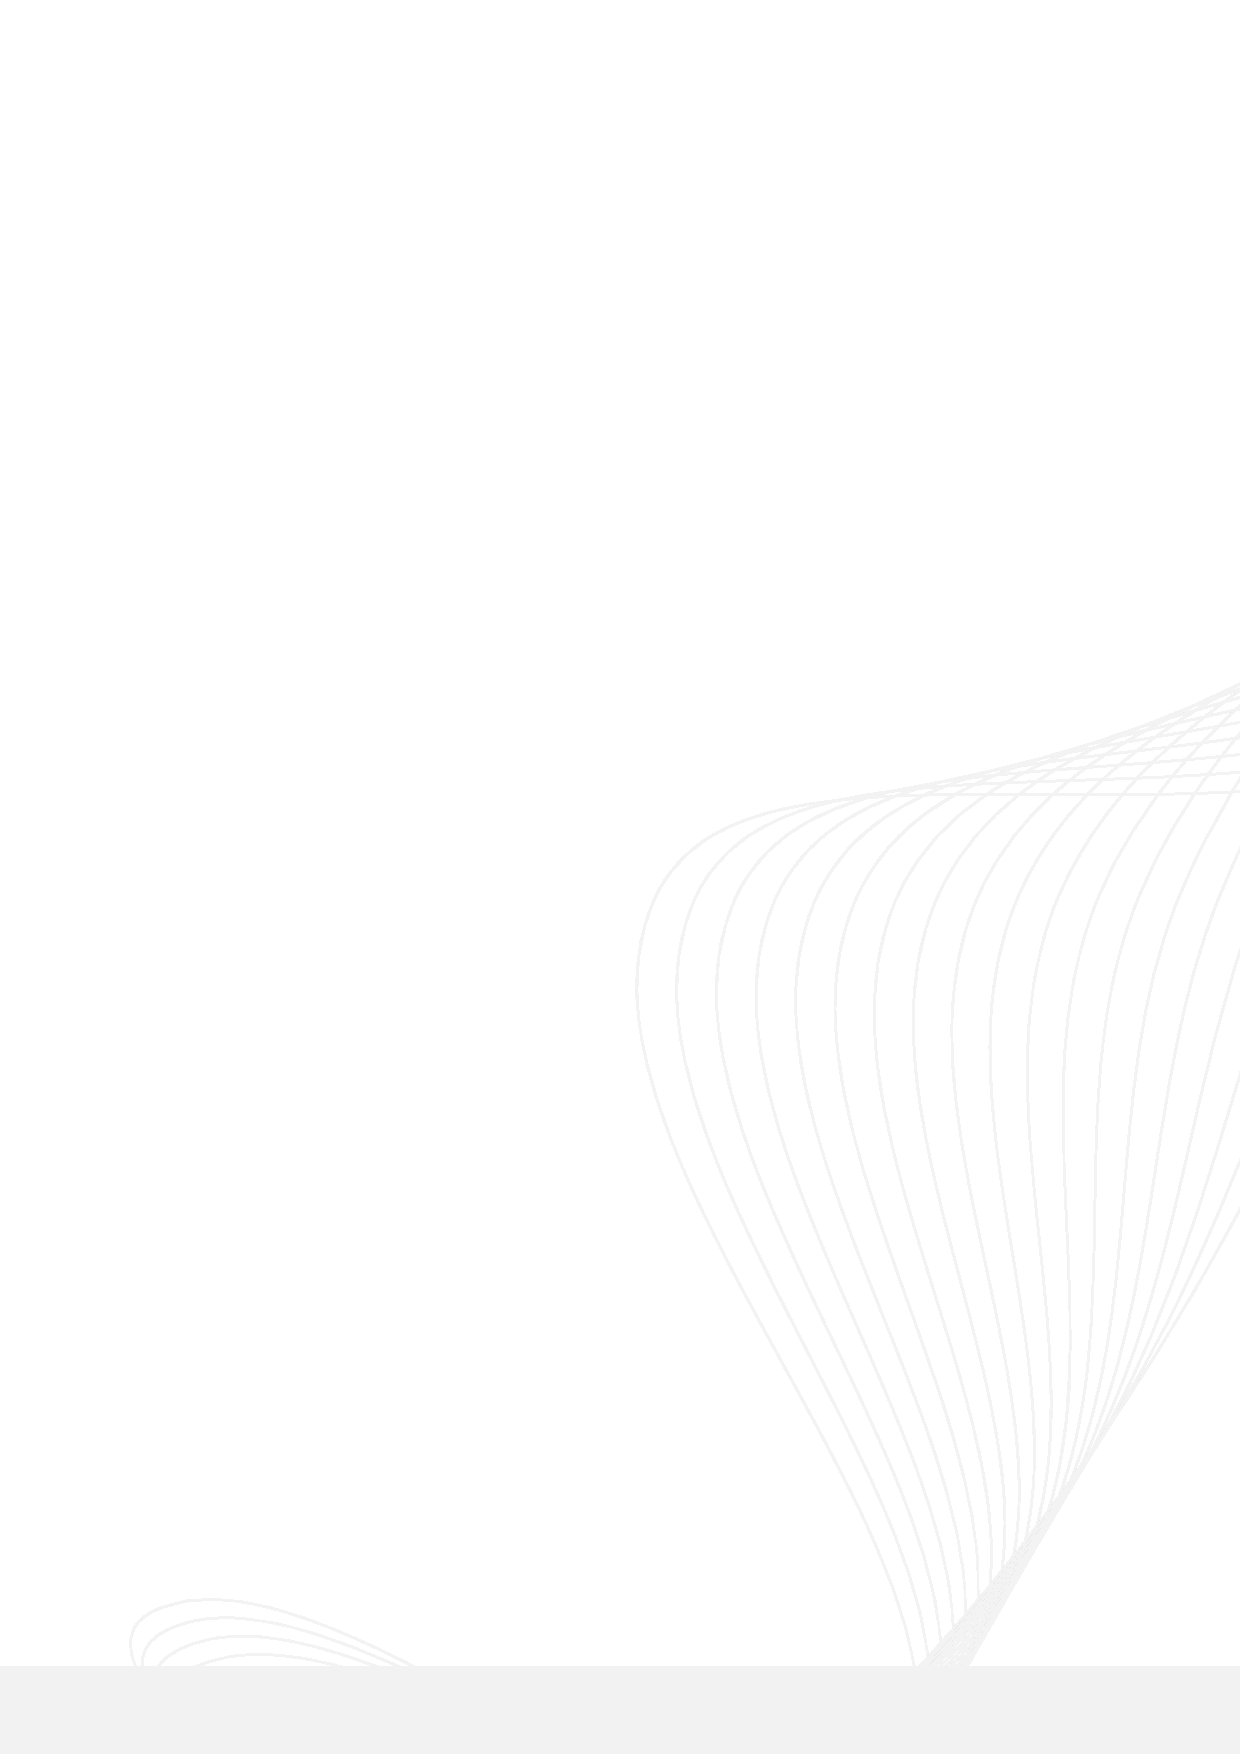
\includegraphics[width=\paperwidth,height=\paperheight,keepaspectratio]{Figures/Theme/Front-Page-BG.pdf}%
    \vfill
    }}}
}

\AddToShipoutPictureBG*{\BackgroundPicCover}

\newgeometry{margin=1.98cm, top=2.15cm, bottom=1.47cm}
\begin{titlepage}
    \latofont
    \ifthenelse{\equal{\CoverOption}{classic}}{\color{white}}{\color{frontpagedark}}
    \vspace*{\baselineskip}

    \ifthenelse{\equal{\CoverOption}{classic}}{
        \ifthenelse{\equal{\SchoolOption}{estg}}{
            \begin{figure}
                
\includegraphics[width=0.485\linewidth]{Figures/Theme/Logotypes/uc-logo-w.png}
            \end{figure}
        }{}

        
        
        \ifthenelse{\equal{\SchoolOption}{esad}}{
            \begin{figure}
                
\includegraphics[width=0.485\linewidth]{Figures/Theme/Logotypes/IPLeiria-ESAD-Logo-W.pdf}
            \end{figure}
        }{}
        
        \ifthenelse{\equal{\SchoolOption}{esslei}}{
            \begin{figure}
                
\includegraphics[width=0.485\linewidth]{Figures/Theme/Logotypes/IPLeiria-ESSLEI-Logo-W.pdf}
            \end{figure}
        }{}
        
        \ifthenelse{\equal{\SchoolOption}{estm}}{
            \begin{figure}
                
\includegraphics[width=0.485\linewidth]{Figures/Theme/Logotypes/IPLeiria-ESTM-Logo-W.pdf}
            \end{figure}
        }{}
        
        \ifthenelse{\equal{\SchoolOption}{esecs}}{
            \begin{figure}
                
\includegraphics[width=0.485\linewidth]{Figures/Theme/Logotypes/IPLeiria-ESECS-Logo-W.pdf}
            \end{figure}
        }{}

    } {
        \ifthenelse{\equal{\SchoolOption}{estg}}{
            \begin{figure}
                
\includegraphics[width=0.485\linewidth]{Figures/Theme/Logotypes/IPLeiria-ESTG-Logo-B.pdf}
                
\includegraphics[width=0.4\linewidth]{Figures/Theme/Logotypes/IPLeiria-ESTG-Logo-Old.png}
            \end{figure}
        }{}
        
        \ifthenelse{\equal{\SchoolOption}{esad}}{
            \begin{figure}
                
\includegraphics[width=0.485\linewidth]{Figures/Theme/Logotypes/IPLeiria-ESAD-Logo-B.pdf}
            \end{figure}
        }{}
        
        \ifthenelse{\equal{\SchoolOption}{esslei}}{
            \begin{figure}
                
\includegraphics[width=0.485\linewidth]{Figures/Theme/Logotypes/IPLeiria-ESSLEI-Logo-B.pdf}
            \end{figure}
        }{}
        
        \ifthenelse{\equal{\SchoolOption}{estm}}{
            \begin{figure}
                
\includegraphics[width=0.485\linewidth]{Figures/Theme/Logotypes/IPLeiria-ESTM-Logo-B.pdf}
            \end{figure}
        }{}
        
        \ifthenelse{\equal{\SchoolOption}{esecs}}{
            \begin{figure}
                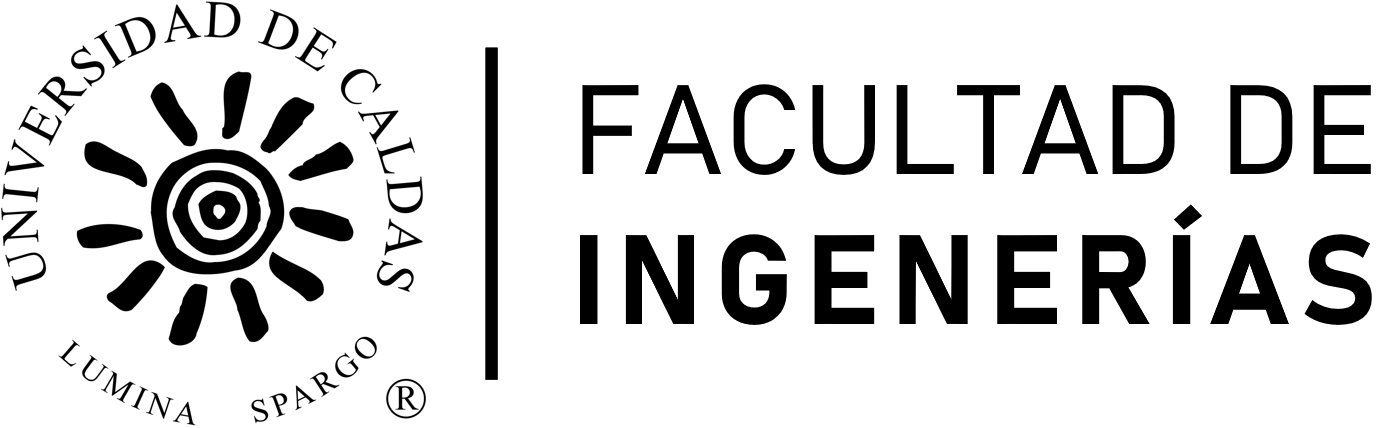
\includegraphics[width=0.485\linewidth]{Figures/Theme/Logotypes/uc-logo-b.png}
            \end{figure}
        }{}
    }

    \vspace{5.5\baselineskip}

    % Title.
	\noindent
    \makebox[\textwidth][l]{%
        \parbox{\dimexpr\textwidth-4cm\relax}{
            \setstretch{1.03}
            \raggedright\bfseries\fontsize{20}{26}\selectfont\GetTitle
        }
    }

    \vspace{0.8\baselineskip}

    % Subtitle.
    \noindent
    \makebox[\textwidth][l]{%
        \parbox{\dimexpr\textwidth-7cm\relax}{
            \setstretch{1.03}
            \raggedright\fontsize{14}{19}\selectfont\GetSubtitle
        }
    }

    \vspace{35pt}  

    % Author.
    {\noindent\bfseries\fontsize{14}{19}\selectfont\GetFirstAuthor}

    \ifdefined\GetSecondAuthor
        \vspace{8pt}
        {\noindent\bfseries\fontsize{14}{19}\selectfont\GetSecondAuthor}
	\fi

    \ifdefined\GetThirdAuthor
        \vspace{8pt}
        {\noindent\bfseries\fontsize{14}{19}\selectfont\GetThirdAuthor}
	\fi
 
	\vfill

    % School.
	{\noindent\fontsize{10}{12}\selectfont\GetSchool}
	
    % Department.
	{\noindent\fontsize{10}{12}\selectfont\GetDepartment}

    % Degree.
	{\noindent\fontsize{10}{12}\selectfont\GetDegree}

    % Course.
    \ifdefined\GetCourse
        {\noindent\fontsize{10}{12}\selectfont\GetCourse}
	\fi

    \ifthenelse{\equal{\DocStageOption}{working}}{
        \vspace{62pt}
        {\noindent\fontsize{10}{12}\selectfont\overwritecolor{yellow}{\GetDocumentVersion \\ \textit{\today}}} 
        \vspace{62pt}
    }{
        \vspace{125pt}
    }

    % Local & Date.
	{\noindent\fontsize{10}{12}\selectfont\GetDate}

    \vspace{68pt}
\end{titlepage}
\restoregeometry
\MediaOptionLogicBlank
\newcommand\BackgroundPicFrontPage{%
    \put(0,0){%
    \parbox[b][\paperheight]{\paperwidth}{%
    \vfill
    \centering
    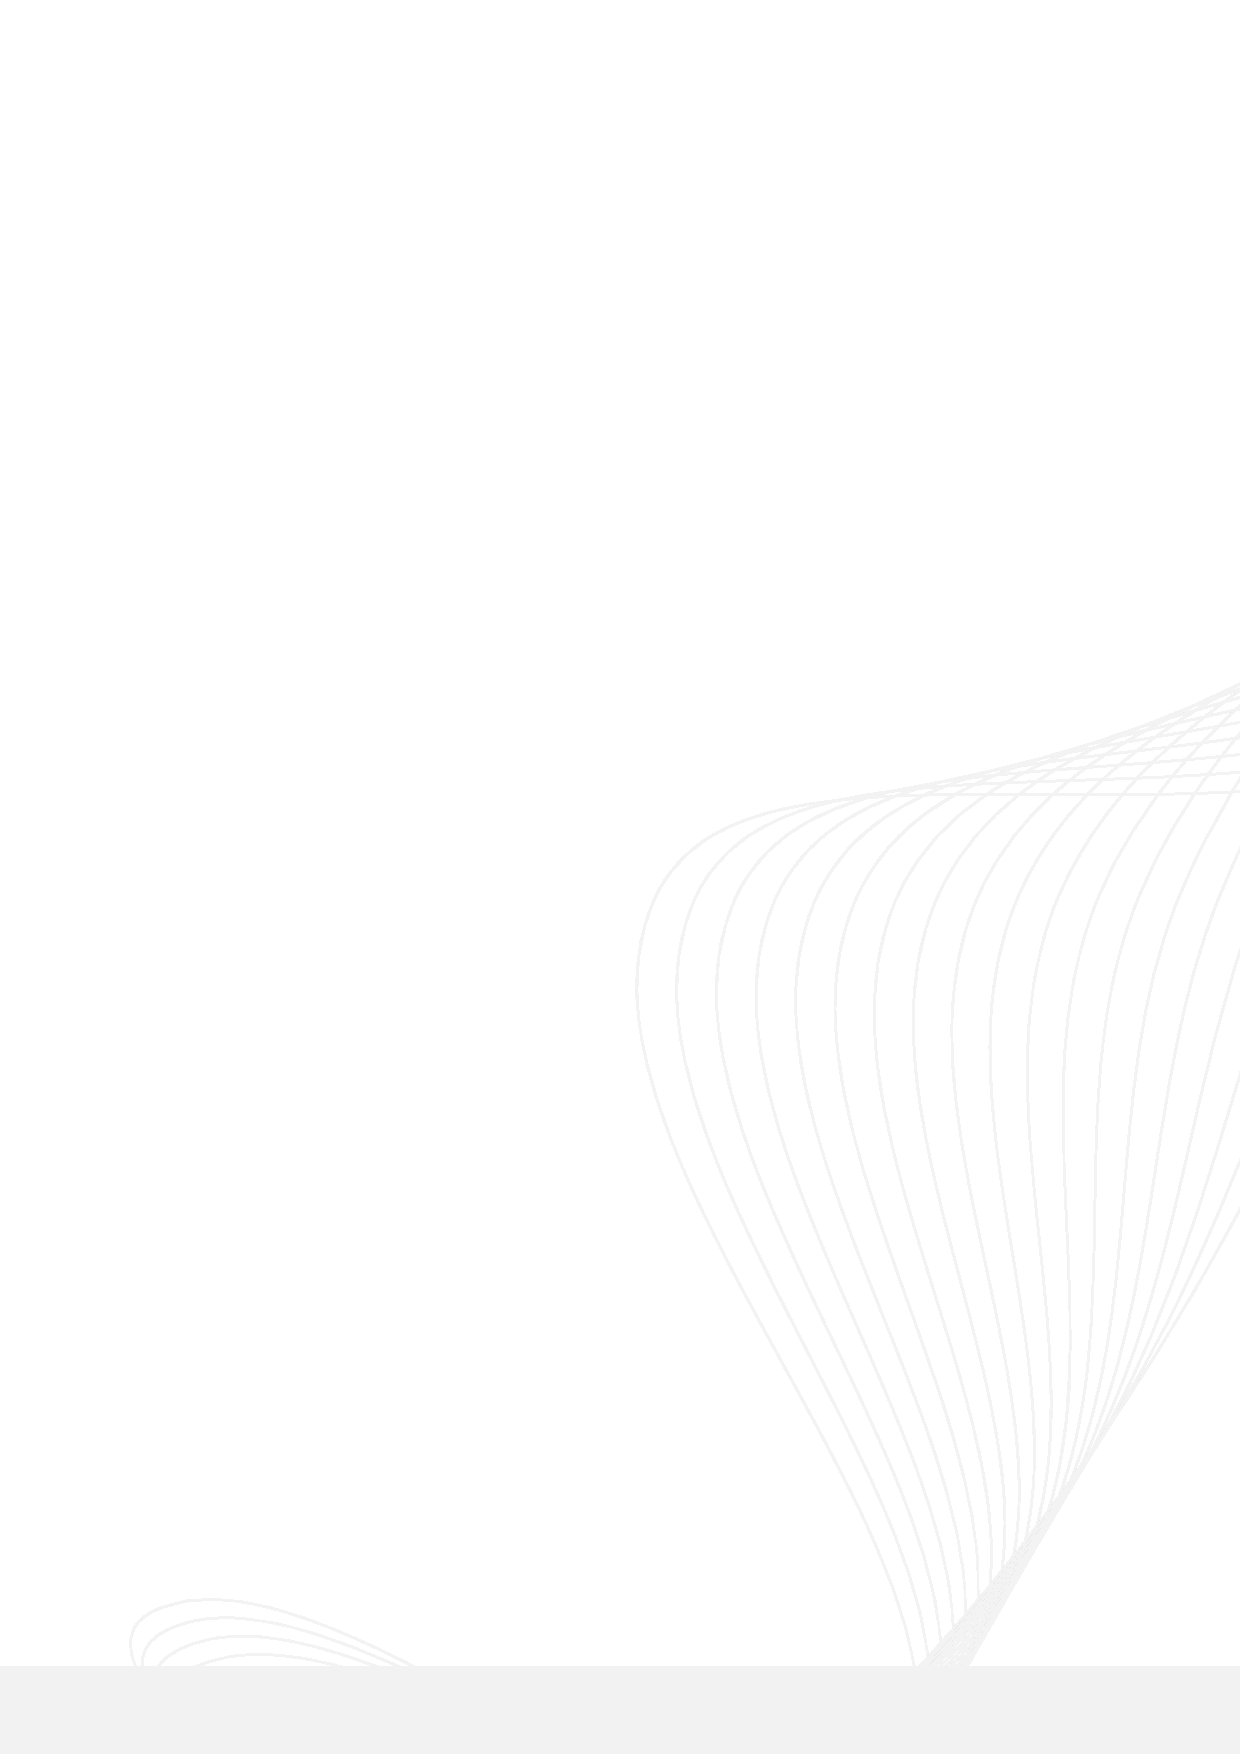
\includegraphics[width=\paperwidth,height=\paperheight,keepaspectratio]{Figures/Theme/Front-Page-BG.pdf}%
    \vfill
}}}
\AddToShipoutPictureBG*{\BackgroundPicFrontPage}

\newgeometry{margin=1.98cm, top=2.15cm, bottom=1.47cm}
\begin{titlepage}
    \latofont
    \color{frontpagedark}
    \vspace*{\baselineskip}

    \ifthenelse{\equal{\SchoolOption}{estg}}{
        \begin{figure}
            % 
\includegraphics[width=0.485\linewidth]{Figures/Theme/Logotypes/IPLeiria-ESTG-Logo-B.pdf}
            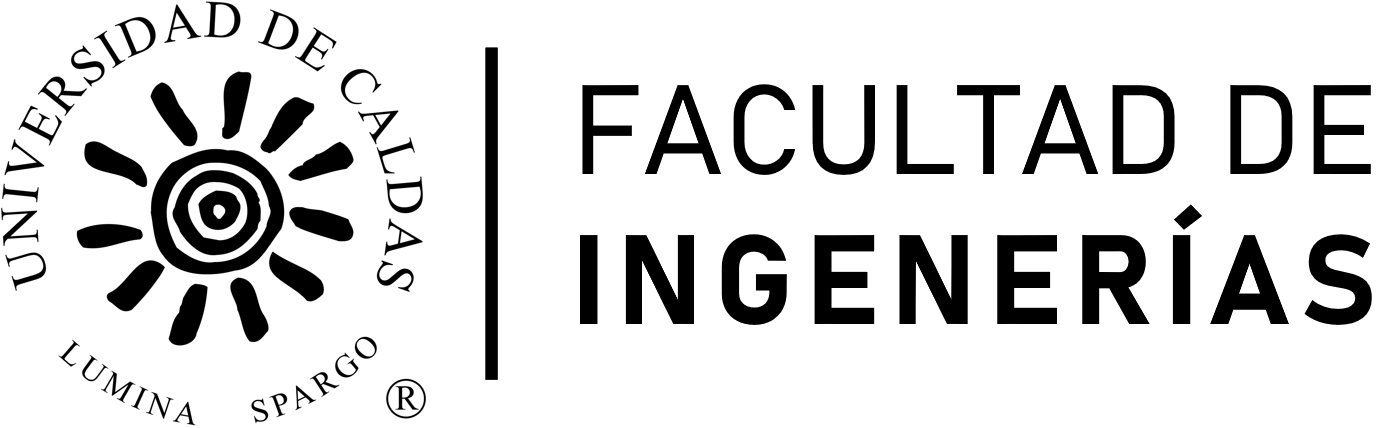
\includegraphics[width=0.4\linewidth]{Figures/Theme/Logotypes/uc-logo-b.png}
        \end{figure}
    }
    
    % \ifthenelse{\equal{\SchoolOption}{esad}}{
    %     \begin{figure}
    %         
\includegraphics[width=0.485\linewidth]{Figures/Theme/Logotypes/IPLeiria-ESAD-Logo-B.pdf}
    %     \end{figure}
    % }
    
    % \ifthenelse{\equal{\SchoolOption}{esslei}}{
    %     \begin{figure}
    %         
\includegraphics[width=0.485\linewidth]{Figures/Theme/Logotypes/IPLeiria-ESSLEI-Logo-B.pdf}
    %     \end{figure}
    % }
    
    % \ifthenelse{\equal{\SchoolOption}{estm}}{
    %     \begin{figure}
    %         
\includegraphics[width=0.485\linewidth]{Figures/Theme/Logotypes/IPLeiria-ESTM-Logo-B.pdf}
    %     \end{figure}
    % }
    
    % \ifthenelse{\equal{\SchoolOption}{esecs}}{
    %     \begin{figure}
    %         
\includegraphics[width=0.485\linewidth]{Figures/Theme/Logotypes/IPLeiria-ESECS-Logo-B.pdf}
    %     \end{figure}
    % }

    \vspace{3.5\baselineskip}

    % Title.
	\noindent
    \makebox[\textwidth][l]{%
        \parbox{\dimexpr\textwidth-2.5cm\relax}{
            \setstretch{1.03}
            \raggedright\bfseries\fontsize{20}{26}\selectfont\GetTitle
        }
    }

    \vspace{0.8\baselineskip}

    % Subtitle.
    % \noindent
    % \makebox[\textwidth][l]{%
    %     \parbox{\dimexpr\textwidth-7cm\relax}{
    %         \setstretch{1.03}
    %         \raggedright\fontsize{14}{19}\selectfont\GetSubtitle
    %     }
    % }

    \vspace{35pt}

    % Author.
    {\noindent\bfseries\fontsize{14}{19}\selectfont\GetFirstAuthor}

    \ifdefined\GetSecondAuthor
        \vspace{8pt}
        {\noindent\bfseries\fontsize{14}{19}\selectfont\GetSecondAuthor}
	\fi

    \ifdefined\GetThirdAuthor
        \vspace{8pt}
        {\noindent\bfseries\fontsize{14}{19}\selectfont\GetThirdAuthor}
	\fi

    \vspace{70pt}    

    {
    \noindent
    \latofont
    \fontsize{10}{12}\selectfont
    \renewcommand{\arraystretch}{0.1}
    \hspace*{-2.5pt}\begin{tabular}{@{}r@{\hspace{5pt}}>{\raggedright\arraybackslash}m{6cm}@{}}
        \textbf{Docente:} & \GetSupervisor \\ [-.7ex]
        & \setstretch{0.9}{\fontsize{8}{10}\selectfont\itshape \GetSupervisorTitle} \\ [2ex]
        
        \ifdefined\GetCoSupervisor
            \textbf{Co-supervisor:} & \GetCoSupervisor \\ [-.7ex]
            & \setstretch{0.9}{\fontsize{8}{10}\selectfont\itshape \GetCoSupervisorTitle} \\ [.5ex]
        \fi

        \ifdefined\GetSecCoSupervisor        
            & \GetSecCoSupervisor \\ [-.7ex]
            & \setstretch{0.9}{\fontsize{8}{10}\selectfont\itshape \GetSecCoSupervisorTitle} \\
        \fi
    \end{tabular}
    }
    
    \vfill
	
    % School.
	{\noindent\fontsize{10}{12}\selectfont\GetSchool}
	
    % Department.
	{\noindent\fontsize{10}{12}\selectfont\GetDepartment}

    % Degree.
	{\noindent\fontsize{10}{12}\selectfont\GetDegree}

    % Course.
    \ifdefined\GetCourse
        {\noindent\fontsize{10}{12}\selectfont\GetCourse}
	\fi

    \vspace{45pt}

    % Thesis option.
	% {\noindent\fontsize{10}{12}\itshape\selectfont\GetThesisType}

    \vspace{45pt}

    % Local and date.
	{\noindent\fontsize{10}{12}\selectfont\GetDate}

    \vspace{68pt}
\end{titlepage}
\restoregeometry
\MediaOptionLogicBlank

%%% Copyright Statement %%%
% \pagenumbering{gobble} % Prevent page numbering.

\vspace*{\fill}

\ifthenelse{\equal{\LanguageOption}{portuguese}}{%
    \noindent \textbf{\GetTitle}
    
    \noindent Copyright \textcopyright~\the\year{} - \GetFirstAuthor, \GetSchool.
    
    \vspace{.575em}
    
    \noindent A presente dissertação é um trabalho original, elaborado exclusivamente para este fim, tendo sido devidamente citados todos os autores cujos estudos contribuíram para a sua elaboração. É permitida a sua reprodução parcial com indicação do autor e referência ao grau, ano letivo, instituição---\textit{Politécnico de Leiria}---e data da defesa pública.

    \vspace{1.395em}
    
    \noindent\psvectorian[scale=.25,opacity=.80]{2}
    
    \vspace{.935em}

    \noindent O presente trabalho beneficiou da utilização do modelo \textit{IPLeiria-Thesis}.
}{%
    \noindent \textbf{\GetTitle}
    
    \noindent Copyright \textcopyright~\the\year{} - \GetFirstAuthor, \GetSchool.
    
    \vspace{.575em}
    
    \noindent This dissertation is original work, written solely for this purpose, and all the authors whose studies and publications contributed to it have been duly cited. Partial reproduction is allowed with acknowledgment of the author and reference to the degree, academic year, institution---\textit{Polytechnic University of Leiria}---and public defense date.

    \vspace{1.395em}
    
    \noindent\psvectorian[scale=.25,opacity=.80]{2}
    
    \vspace{.935em}

    \noindent Preparation of this work was facilitated by the use of the \textit{IPLeiria-Thesis} template.
}

\vspace*{\fill}
\MediaOptionLogic

%%% Roman Numeration %%%
\pagenumbering{roman}

%%% Acknowledgements %%%
% \ifthenelse{\equal{\LanguageOption}{portuguese}}{%
%     \chapter*{Agradecimentos}
% }{%
%     \chapter*{Acknowledgements}
% }

% \guideinfo{In the \textit{Acknowledgment} section, express your gratitude to those who helped and supported your work. Start by thanking your advisors, mentors, or supervisors who provided guidance and expertise. Mention any colleagues, classmates, or team members who contributed to discussions or offered assistance. You can also acknowledge specific organisations, institutions, or funding sources that supported your research or work. Lastly, include any personal acknowledgments for family or friends who offered encouragement and moral support during the project. Keep this section sincere, concise, and professional.}

% \MediaOptionLogicBlank

%%% Abstract %%%
% \thispagestyle{plain}
% \chapter*{Resumo}

% \guiainfo{Na secção \textit{Resumo}, apresente um resumo conciso do seu projeto, destacando os pontos principais. Comece com uma breve declaração do problema ou objetivo, seguido de uma descrição da sua abordagem ou metodologia. Resuma os principais resultados ou conclusões, salientando a sua importância ou implicações. Conclua com uma ou duas frases sobre a contribuição global ou o impacto do seu trabalho. O resumo deve ser claro e conciso, idealmente com 150-250 palavras, para que os leitores compreendam rapidamente o seu trabalho e a sua importância.}

% \keywordspt{Palavra-Chave A, Palavra-Chave B, Palavra-Chave C.}

% \MediaOptionLogicBlank

% \pdfbookmark[1]{Abstract}{abstract}
% \chapter*{Abstract}
% \guideinfo{In the \textit{Abstract} section, provide a concise summary of your project, highlighting the key points. Begin with a brief statement of the problem or objective, followed by a description of your approach or methodology. Summarise the main results or findings, emphasising their significance or implications. Conclude with a sentence or two on the overall contribution or impact of your work. Keep the abstract clear and focused, ideally within 150-250 words, to give readers a quick understanding of your research and its importance.}

% \keywordsen{Keyword A, Keyword B, Keyword C.}

% \MediaOptionLogicBlank

% %%% Table of Contents, List of Figures and List of Tables %%%
\bookmarktocentry\tableofcontents
% \listoffigures
% \listoftables

%%% Print: Glossary and Acronyms %%%
% \glossarytoc\printnormalglossary
% \acronymtoc\printacronymglossary

%%% Arabic Numeration %%%
\pagenumbering{arabic}

%%% Chapters (**Insert Yours Here**) %%%
\chapter[Planteamientos]{Planteamientos}
% \label{cp:introduction}

{
\parindent0pt

\vspace{.935em}

\section{Problema 1 (40\%)}
Con base en la arquitectura definida en la Figura, modelar un conjunto de reglas vía NetFilter/IPTables, así:


\begin{figure}
    \centering
    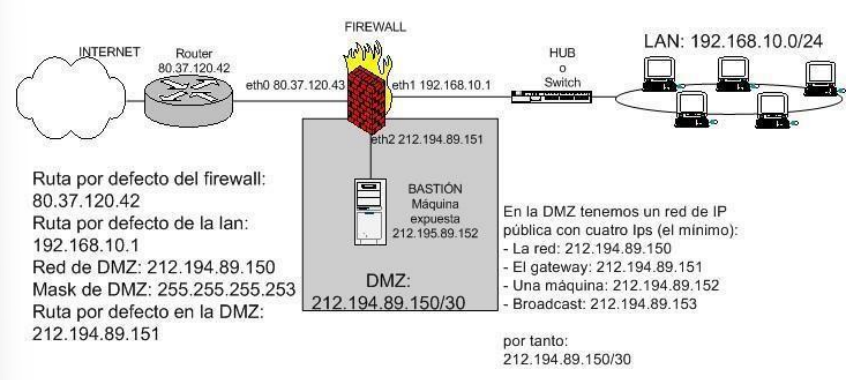
\includegraphics[width=0.5\linewidth]{topologia.png}
    \caption{Topología de red}
    \label{fig:arquitectura-de-red}
\end{figure}


\subsection{Análisis de la Arquitectura de Red}

Analizando la arquitectura mostrada, parece que se presenta la topología clásica de \textbf{defensa en profundidad} con las tres zonas de seguridad claramente diferenciadas:

\begin{itemize}
    \item \textbf{Internet (Zona no confiable):} IP pública del router: 80.37.120.42
    \item \textbf{DMZ (Zona semi-confiable):} Red 212.194.89.150/30
    \begin{itemize}
        \item Gateway: 212.194.89.151 (interfaz eth2 del firewall)
        \item Servidor expuesto: 212.194.89.152
        \item Broadcast: 212.194.89.153
    \end{itemize}
    \item \textbf{LAN Interna (Zona confiable):} Red 192.168.10.0/24
    \begin{itemize}
        \item Gateway: 192.168.10.1 (interfaz eth1 del firewall)
    \end{itemize}
\end{itemize}

\textbf{Interfaces del Firewall:}
\begin{itemize}
    \item \texttt{eth0}: 80.37.120.43 (interfaz externa hacia Internet)
    \item \texttt{eth1}: 192.168.10.1 (interfaz interna hacia LAN)
    \item \texttt{eth2}: 212.194.89.151 (interfaz DMZ)
\end{itemize}



\subsection{Literal a}

\textbf{Permitir el tráfico de los clientes LAN a los Web Servers de la DMZ (*.151, *.152):}

% \subsubsection{Literal A: Permitir tráfico LAN → DMZ (Web Servers)}

Para permitir el acceso desde la red LAN hacia los servidores web en la DMZ, implementamos las siguientes reglas:

\begin{lstlisting}[language=bash, caption=Reglas para tráfico LAN hacia DMZ]
# Permitir HTTP (puerto 80) desde LAN hacia servidor DMZ .151
iptables -A FORWARD -s 192.168.10.0/24 -d 212.194.89.151 \
         -p tcp --dport 80 -m state --state NEW,ESTABLISHED -j ACCEPT

# Permitir HTTP (puerto 80) desde LAN hacia servidor DMZ .152
iptables -A FORWARD -s 192.168.10.0/24 -d 212.194.89.152 \
         -p tcp --dport 80 -m state --state NEW,ESTABLISHED -j ACCEPT

# Permitir HTTPS (puerto 443) desde LAN hacia servidor DMZ .151
iptables -A FORWARD -s 192.168.10.0/24 -d 212.194.89.151 \
         -p tcp --dport 443 -m state --state NEW,ESTABLISHED -j ACCEPT

# Permitir HTTPS (puerto 443) desde LAN hacia servidor DMZ .152
iptables -A FORWARD -s 192.168.10.0/24 -d 212.194.89.152 \
         -p tcp --dport 443 -m state --state NEW,ESTABLISHED -j ACCEPT

# Permitir DNS TCP desde LAN hacia servidores DMZ
iptables -A FORWARD -s 192.168.10.0/24 -d 212.194.89.151 \
         -p tcp --dport 53 -m state --state NEW,ESTABLISHED -j ACCEPT
iptables -A FORWARD -s 192.168.10.0/24 -d 212.194.89.152 \
         -p tcp --dport 53 -m state --state NEW,ESTABLISHED -j ACCEPT

# Permitir DNS UDP desde LAN hacia servidores DMZ
iptables -A FORWARD -s 192.168.10.0/24 -d 212.194.89.151 \
         -p udp --dport 53 -m state --state NEW,ESTABLISHED -j ACCEPT
iptables -A FORWARD -s 192.168.10.0/24 -d 212.194.89.152 \
         -p udp --dport 53 -m state --state NEW,ESTABLISHED -j ACCEPT
\end{lstlisting}

\textbf{Justificación técnica:}
\begin{itemize}
    \item Utilizamos el módulo \texttt{state} con \texttt{NEW,ESTABLISHED} para permitir conexiones nuevas y establecidas.
    \item Se incluyen tanto HTTP (80) como HTTPS (443) para soportar tráfico web seguro.
    \item DNS (53) se permite en TCP y UDP para resolución de nombres completa.
    \item Las reglas son específicas por dirección IP de destino para mayor control.
\end{itemize}

\subsection{Literal b}
\textbf{Permitir el tráfico desde Internet hacia los servidores de la DMZ WWW \& email Server}

% \subsubsection{Literal B: Permitir tráfico Internet → DMZ (WWW \& Email)}

Para exponer los servicios públicos de la DMZ a Internet:

\begin{lstlisting}[language=bash, caption=Reglas para servicios públicos en DMZ]
# === SERVICIOS WEB ===
# Permitir HTTP desde Internet hacia ambos servidores web DMZ
iptables -A FORWARD -i eth0 -d 212.194.89.151 \
         -p tcp --dport 80 -m state --state NEW,ESTABLISHED -j ACCEPT
iptables -A FORWARD -i eth0 -d 212.194.89.152 \
         -p tcp --dport 80 -m state --state NEW,ESTABLISHED -j ACCEPT

# Permitir HTTPS desde Internet hacia ambos servidores web DMZ
iptables -A FORWARD -i eth0 -d 212.194.89.151 \
         -p tcp --dport 443 -m state --state NEW,ESTABLISHED -j ACCEPT
iptables -A FORWARD -i eth0 -d 212.194.89.152 \
         -p tcp --dport 443 -m state --state NEW,ESTABLISHED -j ACCEPT

# === SERVICIOS DE EMAIL (asumiendo .152 como servidor de correo) ===
# SMTP estándar (puerto 25)
iptables -A FORWARD -i eth0 -d 212.194.89.152 \
         -p tcp --dport 25 -m state --state NEW,ESTABLISHED -j ACCEPT

# SMTP seguro - SMTPS (puerto 465)
iptables -A FORWARD -i eth0 -d 212.194.89.152 \
         -p tcp --dport 465 -m state --state NEW,ESTABLISHED -j ACCEPT

# SMTP con STARTTLS (puerto 587)
iptables -A FORWARD -i eth0 -d 212.194.89.152 \
         -p tcp --dport 587 -m state --state NEW,ESTABLISHED -j ACCEPT

# IMAP (puerto 143) e IMAPS (puerto 993)
iptables -A FORWARD -i eth0 -d 212.194.89.152 \
         -p tcp --dport 143 -m state --state NEW,ESTABLISHED -j ACCEPT
iptables -A FORWARD -i eth0 -d 212.194.89.152 \
         -p tcp --dport 993 -m state --state NEW,ESTABLISHED -j ACCEPT

# POP3 (puerto 110) y POP3S (puerto 995)
iptables -A FORWARD -i eth0 -d 212.194.89.152 \
         -p tcp --dport 110 -m state --state NEW,ESTABLISHED -j ACCEPT
iptables -A FORWARD -i eth0 -d 212.194.89.152 \
         -p tcp --dport 995 -m state --state NEW,ESTABLISHED -j ACCEPT
\end{lstlisting}

\textbf{Justificación técnica:}
\begin{itemize}
    \item Se especifica la interfaz de entrada \texttt{-i eth0} para asegurar que el tráfico provenga de Internet.
    \item Se incluyen todos los protocolos de correo estándar (SMTP, IMAP, POP3) y sus versiones seguras.
    \item Las reglas utilizan el módulo de estado para mantener el seguimiento de conexiones.
\end{itemize}


\subsection{Literal c}
\textbf{Proteger el Router de la DMZ y de la LAN para tráfico ICMP y Telnet:}

% \subsection{Literal C: Proteger el Router de la DMZ y LAN (ICMP y Telnet)}

Para proteger el router de accesos no autorizados:

\begin{lstlisting}[language=bash, caption=Reglas de protección del router]
# === BLOQUEO DE TELNET ===
# Bloquear Telnet desde DMZ hacia el router
iptables -A FORWARD -s 212.194.89.150/30 -d 80.37.120.42 \
         -p tcp --dport 23 -j DROP

# Bloquear Telnet desde LAN hacia el router
iptables -A FORWARD -s 192.168.10.0/24 -d 80.37.120.42 \
         -p tcp --dport 23 -j DROP

# === PROTECCIÓN ICMP ===
# Limitar ICMP echo-request (ping) desde DMZ - Anti-DoS
iptables -A FORWARD -s 212.194.89.150/30 -d 80.37.120.42 \
         -p icmp --icmp-type echo-request \
         -m limit --limit 1/s --limit-burst 3 -j ACCEPT

# Limitar ICMP echo-request (ping) desde LAN - Anti-DoS
iptables -A FORWARD -s 192.168.10.0/24 -d 80.37.120.42 \
         -p icmp --icmp-type echo-request \
         -m limit --limit 1/s --limit-burst 3 -j ACCEPT

# Permitir ICMP echo-reply desde DMZ
iptables -A FORWARD -s 212.194.89.150/30 -d 80.37.120.42 \
         -p icmp --icmp-type echo-reply -j ACCEPT

# Permitir ICMP echo-reply desde LAN
iptables -A FORWARD -s 192.168.10.0/24 -d 80.37.120.42 \
         -p icmp --icmp-type echo-reply -j ACCEPT

# Bloquear todos los demás tipos de ICMP hacia el router
iptables -A FORWARD -d 80.37.120.42 -p icmp -j DROP

# === LOGGING PARA ANÁLISIS FORENSE ===
# Registrar intentos de Telnet bloqueados
iptables -A FORWARD -d 80.37.120.42 -p tcp --dport 23 \
         -j LOG --log-prefix "TELNET_BLOCKED_TO_ROUTER: " \
         --log-level 4
\end{lstlisting}

\textbf{Justificación técnica:}
\begin{itemize}
    \item \textbf{Bloqueo de Telnet:} Se deniega completamente el acceso Telnet (puerto 23) por ser un protocolo inseguro.
    \item \textbf{Limitación ICMP:} Se implementa rate limiting (1 ping/segundo) para prevenir ataques DoS.
    \item \textbf{Logging:} Se registran intentos de acceso no autorizado para análisis posterior.
\end{itemize}



\subsection{Literal d}

\textbf{Precisar semánticamente una regla en de Detección de Intrusiones (basada en Snort) que permita alertar intentos de elevar privilegios ( “sudo -i” ) a cualquier servidor de la DMZ:}

% \subsection{Literal D: Regla Snort para Detección de Elevación de Privilegios}

\subsubsection{Regla Principal}

\begin{lstlisting}[language=snort, caption=Regla Snort para detectar sudo -i]
# Regla principal para detectar "sudo -i" en tráfico hacia servidores DMZ
alert tcp any any -> 212.194.89.150/30 any (
    msg:"PRIVILEGE_ESCALATION: Intento de elevacion de privilegios detectado (sudo -i)";
    content:"sudo -i";
    nocase;
    classtype:attempted-admin;
    priority:1;
    sid:1000001;
    rev:1;
    reference:url,cve.mitre.org/cgi-bin/cvename.cgi?name=CVE-2021-3156;
)
\end{lstlisting}

\subsubsection{Análisis Semántico de la Regla}

La regla Snort implementada tiene los siguientes componentes semánticos:

\begin{itemize}
    \item \textbf{Encabezado de la regla:}
    \begin{itemize}
        \item \texttt{alert}: Acción a tomar cuando se detecta la coincidencia.
        \item \texttt{tcp}: Protocolo a monitorear.
        \item \texttt{any any}: Cualquier IP y puerto de origen.
        \item \texttt{-> 212.194.89.150/30 any}: Destino específico en la red DMZ, cualquier puerto.
    \end{itemize}
    
    \item \textbf{Opciones de detección:}
    \begin{itemize}
        \item \texttt{content:"sudo -i"}: Busca la cadena específica en el payload.
        \item \texttt{nocase}: Hace la búsqueda insensible a mayúsculas/minúsculas.
        \item \texttt{classtype:attempted-admin}: Categoriza el evento como intento administrativo.
        \item \texttt{priority:1}: Asigna máxima prioridad (crítico).
        \item \texttt{sid:1000001}: Identificador único de la regla.
        \item \texttt{rev:1}: Versión de la regla.
        \item \texttt{reference}: Enlace a CVE relacionado con vulnerabilidades de sudo.
    \end{itemize}
\end{itemize}

\subsubsection{Reglas Complementarias}

\begin{lstlisting}[language=snort, caption=Reglas adicionales para detección completa]
# Detección de variantes de sudo con expresiones regulares
alert tcp any any -> 212.194.89.150/30 any (
    msg:"PRIVILEGE_ESCALATION: Comando sudo con opciones privilegiadas";
    content:"sudo";
    nocase;
    pcre:"/sudo\s+(-i|--login|-s|--shell|-u\s+root)/i";
    classtype:attempted-admin;
    priority:2;
    sid:1000002;
    rev:1;
)

# Detección de comando su (cambio a root)
alert tcp any any -> 212.194.89.150/30 any (
    msg:"PRIVILEGE_ESCALATION: Intento de cambio a usuario root";
    content:"su -";
    nocase;
    classtype:attempted-admin;
    priority:2;
    sid:1000003;
    rev:1;
)

# Detección de modificación de sudoers
alert tcp any any -> 212.194.89.150/30 any (
    msg:"PRIVILEGE_ESCALATION: Modificacion de archivo sudoers";
    content:"visudo";
    nocase;
    classtype:attempted-admin;
    priority:1;
    sid:1000004;
    rev:1;
)

# Regla avanzada con control de flujo y límite de detección
alert tcp any any -> 212.194.89.150/30 any (
    msg:"PRIVILEGE_ESCALATION: Múltiples intentos de sudo detectados";
    content:"sudo";
    nocase;
    flow:to_server,established;
    threshold:type limit, track by_src, count 3, seconds 60;
    classtype:attempted-admin;
    priority:1;
    sid:1000005;
    rev:1;
)
\end{lstlisting}

\subsubsection{Limitaciones y Consideraciones}

\begin{enumerate}
    \item \textbf{Evasión por codificación:} Los atacantes pueden codificar comandos en base64 o usar ofuscación.
    \item \textbf{Tráfico cifrado:} No detectará comandos dentro de sesiones SSH o HTTPS.
    \item \textbf{Falsos positivos:} Puede alertar sobre uso legítimo de sudo por administradores.
    \item \textbf{Rendimiento:} Las reglas con PCRE pueden impactar el rendimiento en redes de alto tráfico.
\end{enumerate}

% \subsection{Script Completo de Configuración}

% \begin{lstlisting}[language=bash, caption=Script completo de configuración del firewall]
% #!/bin/bash
% # Script de configuración Netfilter/Iptables para arquitectura DMZ
% # Fecha: Junio 2025

% echo "Configurando reglas de firewall para arquitectura DMZ..."

% # === LIMPIEZA INICIAL ===
% iptables -F
% iptables -X
% iptables -t nat -F
% iptables -t nat -X
% iptables -t mangle -F
% iptables -t mangle -X

% # === POLÍTICAS POR DEFECTO ===
% iptables -P INPUT DROP
% iptables -P FORWARD DROP
% iptables -P OUTPUT ACCEPT

% # === REGLAS BÁSICAS ===
% # Permitir loopback
% iptables -A INPUT -i lo -j ACCEPT
% iptables -A OUTPUT -o lo -j ACCEPT

% # Permitir conexiones establecidas
% iptables -A INPUT -m state --state ESTABLISHED,RELATED -j ACCEPT
% iptables -A FORWARD -m state --state ESTABLISHED,RELATED -j ACCEPT

% # === LITERAL A: LAN -> DMZ ===
% # HTTP/HTTPS
% for port in 80 443; do
%     for server in 212.194.89.151 212.194.89.152; do
%         iptables -A FORWARD -s 192.168.10.0/24 -d $server \
%                  -p tcp --dport $port -m state --state NEW -j ACCEPT
%     done
% done

% # DNS
% for server in 212.194.89.151 212.194.89.152; do
%     iptables -A FORWARD -s 192.168.10.0/24 -d $server \
%              -p tcp --dport 53 -m state --state NEW -j ACCEPT
%     iptables -A FORWARD -s 192.168.10.0/24 -d $server \
%              -p udp --dport 53 -m state --state NEW -j ACCEPT
% done

% # === LITERAL B: INTERNET -> DMZ ===
% # Servicios Web
% for port in 80 443; do
%     for server in 212.194.89.151 212.194.89.152; do
%         iptables -A FORWARD -i eth0 -d $server \
%                  -p tcp --dport $port -m state --state NEW -j ACCEPT
%     done
% done

% # Servicios Email (solo .152)
% for port in 25 465 587 143 993 110 995; do
%     iptables -A FORWARD -i eth0 -d 212.194.89.152 \
%              -p tcp --dport $port -m state --state NEW -j ACCEPT
% done

% # === LITERAL C: PROTECCIÓN DEL ROUTER ===
% # Bloquear Telnet
% iptables -A FORWARD -s 212.194.89.150/30 -d 80.37.120.42 \
%          -p tcp --dport 23 -j DROP
% iptables -A FORWARD -s 192.168.10.0/24 -d 80.37.120.42 \
%          -p tcp --dport 23 -j DROP

% # Limitar ICMP
% for source in "212.194.89.150/30" "192.168.10.0/24"; do
%     iptables -A FORWARD -s $source -d 80.37.120.42 \
%              -p icmp --icmp-type echo-request \
%              -m limit --limit 1/s --limit-burst 3 -j ACCEPT
% done

% # Logging
% iptables -A FORWARD -d 80.37.120.42 -p tcp --dport 23 \
%          -j LOG --log-prefix "TELNET_BLOCKED: " --log-level 4

% # === SEGURIDAD ADICIONAL ===
% # Bloquear DMZ -> LAN
% iptables -A FORWARD -s 212.194.89.150/30 -d 192.168.10.0/24 -j DROP

% # Anti-spoofing
% iptables -A FORWARD -s 192.168.10.0/24 ! -i eth1 -j DROP
% iptables -A FORWARD -s 212.194.89.150/30 ! -i eth2 -j DROP

% # Guardar configuración
% echo "Configuración completada. Guardando reglas..."
% iptables-save > /etc/iptables/rules.v4

% echo "Firewall configurado exitosamente."
% \end{lstlisting}

\subsection{Conclusiones}

La implementación presentada proporciona:

\begin{enumerate}
    \item \textbf{Segmentación efectiva:} Separación clara entre zonas de seguridad con control granular del tráfico.
    \item \textbf{Principio de menor privilegio:} Solo se permite el tráfico estrictamente necesario.
    \item \textbf{Defensa en profundidad:} Múltiples capas de seguridad con firewall stateful y IDS (Snort).
    \item \textbf{Monitoreo y auditoría:} Logging detallado para análisis forense y detección de incidentes.
    \item \textbf{Protección contra ataques comunes:} Anti-spoofing, rate limiting, y bloqueo de protocolos inseguros.
\end{enumerate}

Esta configuración debe complementarse con:
\begin{itemize}
    \item Actualización regular de reglas según nuevas amenazas
    \item Integración con SIEM para correlación de eventos
    \item Pruebas periódicas de penetración
    \item Hardening adicional de los sistemas en la DMZ
    \item Implementación de VPN para acceso remoto seguro
\end{itemize}



\section{Problema 2 (25\%)}

2. (25%)
\subsection{Literal a}
\textbf{Brevemente describa el funcionamiento (fases) de SSL/TLS:}

% \section{Problema 2 (25\%): Criptografía y Certificación Digital}

% \subsection{Literal A: Funcionamiento (Fases) de SSL/TLS}

\subsubsection{Descripción General del Protocolo}

SSL/TLS (Secure Socket Layer/Transport Layer Security) es un protocolo criptográfico que proporciona comunicación segura sobre Internet. El protocolo establece una conexión cifrada entre un cliente (navegador) y un servidor, garantizando confidencialidad, integridad y autenticación de los datos transmitidos.

\subsubsection{Fases del Protocolo SSL/TLS}

\textbf{Fase 1: Handshake (Protocolo de Enlace)}

El handshake SSL/TLS es un proceso de negociación que establece los parámetros de seguridad para la comunicación:

\begin{enumerate}
    \item \textbf{Client Hello:} El cliente inicia enviando un mensaje que incluye:
    \begin{itemize}
        \item Versión de TLS soportada
        \item Valor aleatorio del cliente (client random)
        \item Lista de cipher suites disponibles
        \item Extensiones soportadas
    \end{itemize}
    
    \item \textbf{Server Hello:} El servidor responde con:
    \begin{itemize}
        \item Cipher suite seleccionado
        \item Valor aleatorio del servidor (server random)
        \item Certificado SSL/TLS con clave pública
        \item Solicitud opcional de certificado del cliente
    \end{itemize}
    
    \item \textbf{Verificación del Certificado:} El cliente autentica el certificado del servidor verificando:
    \begin{itemize}
        \item Validez temporal del certificado
        \item Coincidencia con el dominio solicitado
        \item Firma de una Autoridad de Certificación (CA) confiable
        \item Estado de revocación del certificado
    \end{itemize}
    
    \item \textbf{Intercambio de Claves:} Generación del secreto compartido:
    \begin{itemize}
        \item El cliente genera un pre-master secret
        \item Lo cifra con la clave pública del servidor
        \item El servidor lo descifra con su clave privada
        \item Ambos derivan las claves de sesión usando client random, server random y pre-master secret
    \end{itemize}
    
    \item \textbf{Finalización:} Confirmación del handshake:
    \begin{itemize}
        \item Cliente envía mensaje "Finished" cifrado con clave de sesión
        \item Servidor envía mensaje "Finished" cifrado
        \item Se establece el canal seguro
    \end{itemize}
\end{enumerate}

\textbf{Fase 2: Capa de Registro (Record Layer)}

Una vez establecido el handshake, la capa de registro maneja el cifrado simétrico de los datos:

\begin{itemize}
    \item \textbf{Fragmentación:} Los datos se dividen en bloques manejables
    \item \textbf{Compresión:} Aplicación opcional de algoritmos de compresión
    \item \textbf{Autenticación:} Generación de MAC (Message Authentication Code)
    \item \textbf{Cifrado:} Aplicación de cifrado simétrico con las claves de sesión
    \item \textbf{Transmisión:} Envío de los datos cifrados a través de la red
\end{itemize}



\subsection{Literal b}
\textbf{Describa las principales diferencias entre un modelo de certificación basado en PKI
con certificados digitales y el estándar PGP:}

% \subsection{Literal B: PKI vs PGP - Principales Diferencias}

\subsubsection{Modelo PKI (Public Key Infrastructure)}

PKI es una infraestructura jerárquica centralizada que gestiona certificados digitales:

\textbf{Características principales:}
\begin{itemize}
    \item \textbf{Autoridad Central:} Las Autoridades de Certificación (CA) actúan como terceros confiables
    \item \textbf{Estructura Jerárquica:} Modelo de árbol con CA raíz y CA subordinadas
    \item \textbf{Certificados X.509:} Formato estándar que incluye clave pública, identidad y firma de la CA
    \item \textbf{Validación Centralizada:} La confianza se basa en la verificación de la cadena de certificación
    \item \textbf{Gestión Corporativa:} Ideal para organizaciones con políticas de seguridad centralizadas
\end{itemize}

\textbf{Proceso de certificación PKI:}
\begin{enumerate}
    \item Usuario genera par de claves (pública/privada)
    \item Solicita certificado a la CA con su clave pública
    \item CA verifica identidad del solicitante
    \item CA firma el certificado con su clave privada
    \item Certificado se distribuye y puede ser verificado por terceros
\end{enumerate}

\subsubsection{Modelo PGP (Pretty Good Privacy)}

PGP implementa un modelo de "red de confianza" descentralizado:

\textbf{Características principales:}
\begin{itemize}
    \item \textbf{Red de Confianza:} No existe autoridad central, la confianza se construye peer-to-peer
    \item \textbf{Firmas Cruzadas:} Los usuarios firman las claves de otros usuarios para validar identidades
    \item \textbf{Niveles de Confianza:} Sistema graduado de confianza basado en relaciones personales
    \item \textbf{Autogestión:} Cada usuario decide en quién confiar sin intermediarios
    \item \textbf{Flexibilidad Algorítmica:} Soporta múltiples algoritmos (RSA/MD5, DH/SHA-1)
\end{itemize}

\textbf{Proceso de certificación PGP:}
\begin{enumerate}
    \item Usuario A genera par de claves y las publica
    \item Usuario B conoce personalmente a A y verifica su identidad
    \item Usuario B firma la clave pública de A con su clave privada
    \item La firma se agrega al certificado de A
    \item Otros usuarios pueden confiar en A basándose en la firma de B
\end{enumerate}

\subsubsection{Comparación Detallada}

\begin{table}[h]
\centering
\caption{PKI vs PGP: Comparación de Modelos}
\begin{tabular}{|l|l|l|}
\hline
\textbf{Aspecto} & \textbf{PKI} & \textbf{PGP} \\
\hline
\textbf{Estructura} & Jerárquica centralizada & Red de confianza descentralizada \\
\hline
\textbf{Autoridad} & CA como tercero confiable & Sin autoridad central \\
\hline
\textbf{Validación} & Cadena de certificación & Firmas cruzadas de usuarios \\
\hline
\textbf{Escalabilidad} & Alta para organizaciones & Limitada por relaciones personales \\
\hline
\textbf{Costo} & Alto (infraestructura CA) & Bajo (sin infraestructura central) \\
\hline
\textbf{Gestión} & Centralizada y automatizada & Descentralizada y manual \\
\hline
\textbf{Revocación} & CRL/OCSP centralizados & Difícil sin autoridad central \\
\hline
\textbf{Uso típico} & Empresas, e-commerce & Comunicaciones personales \\
\hline
\end{tabular}
\end{table}




\subsection{Literal c}
\textbf{¿Por qué las funciones de hashing son el núcleo de la firmas digitales y del blockchains?}

\subsection{Literal C: Funciones Hash como Núcleo de Firmas Digitales y Blockchain}

\subsubsection{Propiedades Fundamentales de las Funciones Hash}

Las funciones hash son algoritmos matemáticos que transforman datos de cualquier tamaño en una cadena de longitud fija:

\textbf{Propiedades criptográficas esenciales:}
\begin{itemize}
    \item \textbf{Determinismo:} El mismo input siempre produce el mismo hash
    \item \textbf{Eficiencia:} Cálculo rápido del hash para cualquier input
    \item \textbf{Irreversibilidad:} Imposible reconstruir el input original desde el hash
    \item \textbf{Resistencia a colisiones:} Extremadamente difícil encontrar dos inputs con el mismo hash
    \item \textbf{Efecto avalancha:} Pequeños cambios en el input causan cambios drásticos en el hash
\end{itemize}

\subsubsection{Rol en las Firmas Digitales}

Las funciones hash son fundamentales en las firmas digitales por las siguientes razones:

\textbf{1. Eficiencia Computacional}
\begin{itemize}
    \item Firmar directamente documentos grandes sería computacionalmente costoso
    \item El hash reduce cualquier documento a una huella de tamaño fijo (ej: 256 bits para SHA-256)
    \item Se firma el hash en lugar del documento completo, optimizando el proceso
\end{itemize}

\textbf{2. Integridad de Datos}
\begin{itemize}
    \item El hash actúa como "huella digital" única del documento
    \item Cualquier alteración del documento cambia completamente el hash
    \item La verificación de la firma detecta automáticamente modificaciones
\end{itemize}

\textbf{3. Proceso de Firma Digital}
\begin{enumerate}
    \item Se calcula el hash del mensaje original
    \item El hash se cifra con la clave privada del firmante
    \item El resultado cifrado es la firma digital
    \item Para verificar: se descifra la firma con la clave pública y se compara con el hash del mensaje recibido
\end{enumerate}

\subsubsection{Rol en Blockchain}

En blockchain, las funciones hash son el núcleo de la seguridad y funcionalidad:

\textbf{1. Integridad de Bloques}
\begin{itemize}
    \item Cada bloque contiene el hash de todas sus transacciones
    \item Cualquier modificación en una transacción cambia el hash del bloque completo
    \item Esto hace que la manipulación sea inmediatamente detectable
\end{itemize}

\textbf{2. Enlace de Bloques}
\begin{itemize}
    \item Cada bloque incluye el hash del bloque anterior
    \item Esto crea una cadena criptográficamente enlazada
    \item Modificar un bloque histórico requiere recalcular todos los bloques posteriores
\end{itemize}

\textbf{3. Prueba de Trabajo (Proof of Work)}
\begin{itemize}
    \item Los mineros buscan un nonce que produzca un hash con características específicas
    \item Bitcoin usa SHA-256 para este proceso
    \item La dificultad computacional protege la red contra ataques
\end{itemize}

\textbf{4. Merkle Trees}
\begin{itemize}
    \item Estructura de datos que usa hashes para organizar transacciones
    \item Permite verificación eficiente de transacciones sin descargar todo el bloque
    \item El hash raíz representa todas las transacciones del bloque
\end{itemize}




\subsection{Literal d}
\textbf{Diagrame y defina el pipeline para firmar y verificar un mensaje usando
sha256withRSA:}

\subsection{Literal D: Pipeline SHA256withRSA - Firma y Verificación}

\subsubsection{Descripción del Algoritmo}

SHA256withRSA es un esquema de firma digital que combina la función hash SHA-256 con el algoritmo de clave pública RSA. Este método implementa el estándar RSASSA-PKCS1-v1\_5 definido en RFC 3447.

\subsubsection{Diagrama del Pipeline}

\begin{figure}[h]
\centering
\begin{tikzpicture}[
    node distance=1.5cm,
    box/.style={rectangle, draw, minimum width=2.5cm, minimum height=1cm, text centered},
    arrow/.style={->, thick}
]

% Proceso de Firma
\node[box] (msg1) {Mensaje Original};
\node[box, below of=msg1] (hash1) {SHA-256 Hash};
\node[box, below of=hash1] (pad1) {PKCS\#1 Padding};
\node[box, below of=pad1] (rsa1) {Cifrado RSA\\(Clave Privada)};
\node[box, below of=rsa1] (b64_1) {Codificación Base64};
\node[box, below of=b64_1] (sig) {Firma Digital};

% Proceso de Verificación
\node[box, right=8cm of msg1] (msg2) {Mensaje Recibido};
\node[box, below of=msg2] (hash2) {SHA-256 Hash};


\node[box, right=4cm of sig] (sig_recv) {Firma Recibida};
\node[box, above of=sig_recv] (b64_2) {Decodificación Base64};
\node[box, above of=b64_2] (rsa2) {Descifrado RSA\\(Clave Pública)};
\node[box, above of=rsa2] (pad2) {Verificación Padding};
\node[box, above of=pad2] (hash_ext) {Hash Extraído};
\node[box, below of=hash2] (compare) {Comparación};
\node[box, below of=compare] (result) {Resultado\\Verificación};

% Flechas proceso de firma
\draw[arrow] (msg1) -- (hash1);
\draw[arrow] (hash1) -- (pad1);
\draw[arrow] (pad1) -- (rsa1);
\draw[arrow] (rsa1) -- (b64_1);
\draw[arrow] (b64_1) -- (sig);

% Flechas proceso de verificación
\draw[arrow] (msg2) -- (hash2);
\draw[arrow] (sig_recv) -- (b64_2);
\draw[arrow] (b64_2) -- (rsa2);
\draw[arrow] (rsa2) -- (pad2);
\draw[arrow] (pad2) -- (hash_ext);
\draw[arrow] (hash2) -- (compare);
\draw[arrow] (hash_ext) -- (compare);
\draw[arrow] (compare) -- (result);

% Etiquetas
\node[above=1cm of msg1, xshift=1.5cm] {\textbf{PROCESO DE FIRMA}};
\node[above=1cm of msg2, xshift=1.5cm] {\textbf{PROCESO DE VERIFICACIÓN}};

\end{tikzpicture}
\caption{Pipeline SHA256withRSA - Firma y Verificación}
\end{figure}

\subsubsection{Proceso Detallado de Firma}

\textbf{Paso 1: Generación del Hash}
\begin{lstlisting}[language=pseudocode, caption=Cálculo del hash SHA-256]
FUNCTION generateHash(message):
    // Aplicar función hash SHA-256
    hash = SHA256(message)
    // Resultado: 32 bytes (256 bits)
    RETURN hash
END FUNCTION
\end{lstlisting}

\textbf{Paso 2: Aplicación de Padding PKCS\#1}
\begin{lstlisting}[language=pseudocode, caption=Padding PKCS\#1 v1.5]
FUNCTION applyPKCS1Padding(hash, keySize):
    // Identificador de algoritmo SHA-256
    algorithmId = "3031300d060960864801650304020105000420"
    
    // Construir estructura ASN.1
    digestInfo = algorithmId + hash
    
    // Calcular padding necesario
    paddingLength = keySize - length(digestInfo) - 3
    padding = "FF" repetido paddingLength veces
    
    // Construir mensaje con padding
    paddedMessage = "0001" + padding + "00" + digestInfo
    
    RETURN paddedMessage
END FUNCTION
\end{lstlisting}

\textbf{Paso 3: Firma RSA}
\begin{lstlisting}[language=pseudocode, caption=Operación de firma RSA]
FUNCTION signRSA(paddedMessage, privateKey):
    // Convertir mensaje a entero
    m = bytesToInteger(paddedMessage)
    
    // Operación RSA: s = m^d mod n
    // donde d es el exponente privado y n es el módulo
    signature = modularExponentiation(m, privateKey.d, privateKey.n)
    
    // Convertir resultado a bytes
    signatureBytes = integerToBytes(signature, privateKey.keySize)
    
    RETURN signatureBytes
END FUNCTION
\end{lstlisting}

\textbf{Paso 4: Codificación Base64}
\begin{lstlisting}[language=pseudocode, caption=Codificación final]
FUNCTION encodeSignature(signatureBytes):
    // Codificar en Base64 para transmisión
    base64Signature = base64Encode(signatureBytes)
    RETURN base64Signature
END FUNCTION
\end{lstlisting}

\subsubsection{Proceso Detallado de Verificación}

\textbf{Paso 1: Decodificación y Verificación RSA}
\begin{lstlisting}[language=pseudocode, caption=Verificación de firma RSA]
FUNCTION verifyRSA(signature, publicKey):
    // Decodificar Base64
    signatureBytes = base64Decode(signature)
    
    // Convertir a entero
    s = bytesToInteger(signatureBytes)
    
    // Operación RSA inversa: m = s^e mod n
    // donde e es el exponente público
    decrypted = modularExponentiation(s, publicKey.e, publicKey.n)
    
    // Convertir resultado a bytes
    decryptedBytes = integerToBytes(decrypted, publicKey.keySize)
    
    RETURN decryptedBytes
END FUNCTION
\end{lstlisting}

\textbf{Paso 2: Verificación de Padding y Extracción de Hash}
\begin{lstlisting}[language=pseudocode, caption=Extracción del hash original]
FUNCTION extractHash(decryptedBytes):
    // Verificar formato PKCS#1
    IF decryptedBytes[0] != 0x00 OR decryptedBytes[1] != 0x01 THEN
        RETURN ERROR("Invalid PKCS#1 format")
    END IF
    
    // Buscar separador 0x00
    separatorIndex = findByte(decryptedBytes, 0x00, startIndex=2)
    
    // Extraer DigestInfo
    digestInfo = decryptedBytes[separatorIndex+1:]
    
    // Verificar identificador de algoritmo SHA-256
    expectedAlgId = "3031300d060960864801650304020105000420"
    IF NOT startsWith(digestInfo, expectedAlgId) THEN
        RETURN ERROR("Invalid algorithm identifier")
    END IF
    
    // Extraer hash (últimos 32 bytes)
    extractedHash = digestInfo[length(expectedAlgId):]
    
    RETURN extractedHash
END FUNCTION
\end{lstlisting}

\textbf{Paso 3: Comparación Final}
\begin{lstlisting}[language=pseudocode, caption=Verificación de integridad]
FUNCTION verifySignature(message, signature, publicKey):
    // Calcular hash del mensaje recibido
    messageHash = SHA256(message)
    
    // Verificar firma y extraer hash
    extractedHash = extractHash(verifyRSA(signature, publicKey))
    
    // Comparación segura de hashes
    IF secureCompare(messageHash, extractedHash) THEN
        RETURN "SIGNATURE_VALID"
    ELSE
        RETURN "SIGNATURE_INVALID"
    END IF
END FUNCTION
\end{lstlisting}

\subsubsection{Consideraciones de Seguridad}

\textbf{Fortalezas del Esquema:}
\begin{itemize}
    \item \textbf{Resistencia criptográfica:} SHA-256 proporciona 128 bits de seguridad efectiva
    \item \textbf{Estándar probado:} PKCS\#1 v1.5 es ampliamente utilizado y auditado
    \item \textbf{Interoperabilidad:} Compatible con múltiples plataformas y librerías
\end{itemize}

\textbf{Vulnerabilidades Potenciales:}
\begin{itemize}
    \item \textbf{Ataques de padding:} PKCS\#1 v1.5 es susceptible a ataques de padding oracle
    \item \textbf{Tamaño de clave:} RSA requiere claves de al menos 2048 bits para seguridad actual
    \item \textbf{Implementación:} Errores en la implementación pueden comprometer la seguridad
\end{itemize}

\textbf{Mejores Prácticas:}
\begin{itemize}
    \item Usar claves RSA de 2048 bits o superiores
    \item Implementar verificación temporal de certificados
    \item Considerar migración a PSS (Probabilistic Signature Scheme) para mayor seguridad
    \item Implementar protecciones contra ataques de canal lateral
\end{itemize}



















\section{Problema 3 (35\%)}
\textbf{Desarrollo Seguro y DevSecOps:}




\subsection{Literal a}
\textbf{Brevemente describa el funcionamiento (fases) de SSL/TLS:}

% \subsection{Literal A: Inyección SQL - Funcionalidad y Contramedidas}

\subsubsection{Funcionalidad de la Inyección SQL}

La \textbf{inyección SQL} es una técnica de ataque que explota vulnerabilidades en la capa de datos de una aplicación, permitiendo a un atacante ejecutar comandos SQL arbitrarios en la base de datos. Esta vulnerabilidad ocurre cuando la aplicación construye consultas SQL dinámicamente concatenando entrada del usuario sin validación adecuada, haciendo que los datos proporcionados por el usuario se interpreten como código SQL en lugar de datos literales.

El \textbf{mecanismo de funcionamiento} se basa en la inserción directa de código malicioso en variables especificadas por el usuario que se concatenan con comandos SQL y se ejecutan. El proceso típico involucra:

\begin{enumerate}
    \item \textbf{Finalización prematura de cadenas:} El atacante termina una cadena de texto existente
    \item \textbf{Anexión de comandos maliciosos:} Se inserta código SQL no autorizado
    \item \textbf{Uso de comentarios:} Se emplean marcas como \texttt{--} para omitir el resto de la consulta original
\end{enumerate}

\textbf{Ejemplo de vulnerabilidad:}

\begin{lstlisting}[language=SQL, caption=Consulta vulnerable por concatenación]
-- Código original vulnerable
consulta := "SELECT * FROM usuarios WHERE nombre = '" + nombreUsuario + "';"

-- Si el atacante ingresa: Alicia'; DROP TABLE usuarios; --
-- Resulta en:
SELECT * FROM usuarios WHERE nombre = 'Alicia'; 
DROP TABLE usuarios; --';
\end{lstlisting}

\textbf{Tipos principales de inyección SQL:}

\begin{itemize}
    \item \textbf{In-band (Clásica):} Los resultados se obtienen por el mismo canal de comunicación
    \begin{itemize}
        \item \textit{Error-based:} Extrae información mediante mensajes de error de la base de datos
        \item \textit{Union-based:} Combina resultados usando el operador UNION SQL
    \end{itemize}
    
    \item \textbf{Inferential (Blind):} No se obtienen datos directamente, requiere inferencia
    \begin{itemize}
        \item \textit{Boolean-based:} Deduce información según respuestas verdadero/falso
        \item \textit{Time-based:} Usa delays temporales para inferir información
    \end{itemize}
    
    \item \textbf{Out-of-band:} Exfiltra datos por un canal diferente (HTTP, DNS, etc.)
\end{itemize}

\subsubsection{Contramedidas contra Inyección SQL}

\textbf{Contramedida 1: Consultas Parametrizadas (Prepared Statements)}

Las consultas parametrizadas separan completamente el código SQL de los datos, haciendo imposible la inyección. Esta técnica utiliza marcadores de posición que asignan mecánicamente valores de entrada a sentencias SQL preparadas previamente.

\begin{lstlisting}[language=SQL, caption=Implementación segura con consultas parametrizadas]
-- Estructura segura con parámetros
PREPARE stmt FROM 'SELECT * FROM users WHERE username = ? AND password = ?';
SET @username = 'valor_usuario';
SET @password = 'valor_password';
EXECUTE stmt USING @username, @password;
DEALLOCATE PREPARE stmt;
\end{lstlisting}

\textbf{Ventajas técnicas:}
\begin{itemize}
    \item Separación absoluta entre código y datos
    \item Prevención automática de inyección SQL
    \item Mejor rendimiento por caché de planes de ejecución
    \item Portabilidad entre diferentes motores de base de datos
\end{itemize}

\textbf{Contramedida 2: Procedimientos Almacenados (Stored Procedures)}

Los procedimientos almacenados encapsulan la lógica SQL en el servidor de base de datos, proporcionando una capa adicional de seguridad. Ejecutan varios comandos SQL en una sola sentencia sin permitir acceso directo al servidor a través de campos de entrada.

\begin{lstlisting}[language=SQL, caption=Procedimiento almacenado seguro]
-- Crear procedimiento almacenado con validación
CREATE PROCEDURE sp_authenticate_user
    @Username NVARCHAR(50),
    @Password NVARCHAR(255)
AS
BEGIN
    -- Validación de entrada dentro del procedimiento
    IF LEN(@Username) > 50 OR LEN(@Password) > 255
    BEGIN
        RAISERROR('Invalid input length', 16, 1)
        RETURN
    END
    
    -- Consulta segura con parámetros
    SELECT user_id, username, role 
    FROM users 
    WHERE username = @Username 
    AND password_hash = HASHBYTES('SHA2_256', @Password + salt)
END
\end{lstlisting}



\subsection{Literal b}
\textbf{Describa las principales diferencias entre un modelo de certificación basado en PKI
con certificados digitales y el estándar PGP:}

% \subsection{Literal B: Controles Mínimos para Desarrollo Seguro}

\subsubsection{Control 1: Gestión Segura de Autenticación y Sesiones}

\textbf{Descripción:} Implementar mecanismos robustos de autenticación que protejan las credenciales y gestionen las sesiones de forma segura.

\textbf{Elementos clave:}
\begin{itemize}
    \item Hash de contraseñas con algoritmos seguros (BCrypt, Argon2)
    \item Protección contra ataques de fuerza bruta mediante rate limiting
    \item Regeneración de ID de sesión para prevenir session fixation
    \item Implementación de tokens CSRF únicos por sesión
    \item Timeout de sesiones y logout seguro
    \item Logging de eventos de autenticación para auditoría
\end{itemize}

\begin{lstlisting}[language=pseudocode, caption=Pseudocódigo para autenticación segura]
FUNCTION authenticateUser(username, password, request):
    // 1. Validar entrada
    IF NOT isValidInput(username, password) THEN
        RETURN AuthResult.failure()
    END IF
    
    // 2. Verificar intentos fallidos (anti brute-force)
    IF isAccountLocked(username) THEN
        logSecurityEvent("LOCKED_ACCOUNT_ACCESS", username)
        THROW AccountLockedException
    END IF
    
    // 3. Verificar contraseña con hash seguro
    user = getUserByUsername(username)
    IF user == NULL OR NOT verifyPassword(password, user.passwordHash) THEN
        incrementFailedAttempts(username)
        RETURN AuthResult.failure()
    END IF
    
    // 4. Generar sesión segura
    session = createSecureSession(user)
    regenerateSessionId(session)
    setCsrfToken(session)
    
    RETURN AuthResult.success(user, session)
END FUNCTION
\end{lstlisting}

\subsubsection{Control 2: Validación y Sanitización de Entrada}

\textbf{Descripción:} Toda entrada externa debe ser validada contra reglas de negocio específicas y sanitizada antes de su procesamiento.

\textbf{Principios fundamentales:}
\begin{itemize}
    \item \textbf{Nunca confiar en datos de entrada:} Todo debe ser verificado para garantizar que corresponde a lo esperado
    \item \textbf{Validación por whitelist:} Definir explícitamente qué caracteres y formatos son permitidos
    \item \textbf{Sanitización contextual:} Aplicar escapado específico según el contexto de uso (HTML, JavaScript, SQL, etc.)
    \item \textbf{Verificación de longitud y formato:} Establecer límites máximos y patrones válidos
    \item \textbf{Detección de patrones peligrosos:} Identificar y bloquear secuencias maliciosas conocidas
\end{itemize}

\begin{lstlisting}[language=pseudocode, caption=Framework de validación de entrada]
FUNCTION validateInput(input, validationContext):
    // 1. Verificar nulos y longitud
    IF input == NULL OR length(input) > validationContext.maxLength THEN
        RETURN ValidationResult.error("Invalid input")
    END IF
    
    // 2. Aplicar reglas de formato
    IF NOT matches(input, validationContext.pattern) THEN
        RETURN ValidationResult.error("Invalid format")
    END IF
    
    // 3. Verificar patrones peligrosos
    dangerousPatterns = ["<script", "javascript:", "union select", "../"]
    FOR EACH pattern IN dangerousPatterns DO
        IF contains(input, pattern) THEN
            logSecurityEvent("DANGEROUS_PATTERN", input)
            RETURN ValidationResult.error("Forbidden pattern")
        END IF
    END FOR
    
    // 4. Sanitizar según contexto
    sanitized = sanitizeForContext(input, validationContext.outputContext)
    RETURN ValidationResult.success(sanitized)
END FUNCTION
\end{lstlisting}

\subsubsection{Control 3: Cifrado de Datos Sensibles}

\textbf{Descripción:} Implementar cifrado tanto en tránsito como en reposo para proteger información confidencial.

\textbf{Componentes esenciales:}
\begin{itemize}
    \item \textbf{Cifrado en tránsito:} Uso de protocolos seguros (TLS 1.3, HTTPS) para todas las comunicaciones
    \item \textbf{Cifrado en reposo:} Protección de datos almacenados usando algoritmos fuertes (AES-256)
    \item \textbf{Gestión segura de claves:} Implementación de HSM o sistemas de gestión de claves dedicados
    \item \textbf{Derivación de claves contextual:} Uso de técnicas como HKDF para generar claves específicas
    \item \textbf{Rotación regular de claves:} Establecer políticas de renovación periódica
\end{itemize}

\begin{lstlisting}[language=pseudocode, caption=Cifrado de datos sensibles]
FUNCTION encryptSensitiveData(plaintext, context):
    // 1. Derivar clave específica del contexto
    contextKey = deriveKey(masterKey, context)
    
    // 2. Generar IV aleatorio
    iv = generateRandomBytes(12) // Para AES-GCM
    
    // 3. Configurar cifrado AES-GCM
    cipher = initializeCipher("AES-GCM", contextKey, iv)
    
    // 4. Agregar datos adicionales autenticados
    aad = context + ":" + currentTimestamp()
    cipher.setAAD(aad)
    
    // 5. Cifrar datos
    ciphertext = cipher.encrypt(plaintext)
    
    // 6. Retornar objeto con metadatos
    RETURN EncryptedData(ciphertext, iv, algorithm, keyVersion, context, aad)
END FUNCTION
\end{lstlisting}

\subsubsection{Control 4: Manejo Seguro de Errores y Logging}

\textbf{Descripción:} Los errores deben manejarse sin exponer información sensible, manteniendo registros detallados para análisis forense.

\textbf{Características principales:}
\begin{itemize}
    \item \textbf{Mensajes de error genéricos:} Evitar revelar detalles técnicos o estructura interna
    \item \textbf{Logging estructurado:} Registro detallado de eventos de seguridad en formato JSON
    \item \textbf{Sanitización de logs:} Redactar información sensible antes del registro
    \item \textbf{Correlación de eventos:} Asignar IDs únicos para trazabilidad de incidentes
    \item \textbf{Alertas automáticas:} Notificación inmediata para eventos críticos de seguridad
\end{itemize}

\begin{lstlisting}[language=pseudocode, caption=Manejo seguro de errores]
FUNCTION handleException(exception, request):
    // 1. Generar ID único para trazabilidad
    errorId = generateUUID()
    
    // 2. Clasificar el error
    classification = classifyError(exception)
    
    // 3. Log detallado (solo interno)
    logContext = {
        "errorId": errorId,
        "timestamp": currentTimestamp(),
        "exception": exception.type,
        "message": exception.message,
        "remoteAddr": request.remoteAddress,
        "userAgent": sanitize(request.userAgent),
        "requestUri": request.uri,
        "parameters": sanitizeParameters(request.parameters)
    }
    securityLogger.error(toJSON(logContext))
    
    // 4. Respuesta genérica al cliente
    clientResponse = createSafeResponse(errorId, classification)
    
    // 5. Notificar si es crítico
    IF classification.isCritical() THEN
        notifySecurityTeam(errorId, exception)
    END IF
    
    RETURN clientResponse
END FUNCTION
\end{lstlisting}





\subsection{Literal c}
\textbf{¿Por qué las funciones de hashing son el núcleo de la firmas digitales y del blockchains?}

% \subsection{Literal C: Enfoques Shift Left vs Shift Right en DevSecOps}

\subsubsection{Shift Left: Seguridad Temprana en el Desarrollo}

\textbf{Definición:} El enfoque Shift Left consiste en incorporar controles de seguridad en las primeras etapas del ciclo de vida del desarrollo de software (SDLC). Se basa en el principio de que es más eficiente y económico detectar y corregir vulnerabilidades durante las fases de diseño y desarrollo que en producción.

\textbf{Características principales:}
\begin{itemize}
    \item \textbf{Integración temprana:} La seguridad se considera desde la planificación y diseño
    \item \textbf{Automatización de pruebas:} Implementación de análisis estático y dinámico en el pipeline CI/CD
    \item \textbf{Desarrollo dirigido por seguridad:} Los desarrolladores reciben herramientas y capacitación en prácticas seguras
    \item \textbf{Detección proactiva:} Identificación de vulnerabilidades antes del despliegue
\end{itemize}

\textbf{Etapas de aplicación en el SDLC:}
\begin{itemize}
    \item \textbf{Planificación:} Definición de requisitos de seguridad y modelado de amenazas
    \item \textbf{Diseño:} Revisión de arquitectura de seguridad y selección de patrones seguros
    \item \textbf{Desarrollo:} Análisis estático de código (SAST) y revisiones de código
    \item \textbf{Pruebas:} Análisis dinámico (DAST) y pruebas de penetración automatizadas
\end{itemize}

\textbf{Ejemplo de herramienta:} \textbf{SonarQube} - Plataforma de análisis estático que se integra en el pipeline CI/CD para detectar vulnerabilidades, code smells y problemas de calidad durante la fase de desarrollo, proporcionando feedback inmediato a los desarrolladores.

\begin{lstlisting}[language=yaml, caption=Integración de SonarQube en pipeline CI/CD]
# Pipeline CI/CD con análisis estático
stages:
  - build
  - security-scan
  - test
  - deploy

sonarqube-scan:
  stage: security-scan
  script:
    - sonar-scanner 
        -Dsonar.projectKey=myproject
        -Dsonar.sources=src/
        -Dsonar.host.url=$SONAR_HOST_URL
        -Dsonar.login=$SONAR_TOKEN
  rules:
    - if: '$CI_COMMIT_BRANCH == "main"'
    - if: '$CI_PIPELINE_SOURCE == "merge_request_event"'
  
quality-gate:
  stage: security-scan
  script:
    - sonar-quality-gate-check
  dependencies:
    - sonarqube-scan
  allow_failure: false  # Bloquea el pipeline si hay vulnerabilidades críticas
\end{lstlisting}

\subsubsection{Shift Right: Seguridad Continua en Producción}

\textbf{Definición:} El enfoque Shift Right se centra en la supervisión continua del comportamiento, rendimiento e indicadores de seguridad durante la etapa de producción. Su objetivo es verificar el funcionamiento real del software y detectar amenazas en tiempo real.

\textbf{Características principales:}
\begin{itemize}
    \item \textbf{Monitoreo continuo:} Supervisión 24/7 de aplicaciones en producción
    \item \textbf{Observabilidad:} Recolección y análisis de métricas, logs y trazas en tiempo real
    \item \textbf{Respuesta a incidentes:} Capacidad de detección y mitigación automática de amenazas
    \item \textbf{Feedback loop:} Información de producción que mejora el desarrollo futuro
\end{itemize}

\textbf{Etapas de aplicación en el SDLC:}
\begin{itemize}
    \item \textbf{Despliegue:} Monitoreo de la implementación y configuración
    \item \textbf{Producción:} Supervisión continua de seguridad y rendimiento
    \item \textbf{Mantenimiento:} Análisis de patrones de uso y detección de anomalías
    \item \textbf{Evolución:} Retroalimentación para mejorar versiones futuras
\end{itemize}

\textbf{Ejemplo de herramienta:} \textbf{Splunk SIEM} - Sistema de gestión de eventos e información de seguridad que correlaciona logs y eventos de múltiples fuentes en tiempo real, detecta patrones anómalos y genera alertas automáticas para respuesta inmediata a incidentes de seguridad en producción.

\begin{lstlisting}[language=spl, caption=Consulta Splunk para detección de anomalías]
# Búsqueda SPL para detectar intentos de inyección SQL
index=webapp sourcetype=access_log
| regex _raw="(?i)(union|select|insert|update|delete|drop|exec)"
| eval threat_level=case(
    match(_raw, "(?i)union.*select"), "HIGH",
    match(_raw, "(?i)drop.*table"), "CRITICAL",
    match(_raw, "(?i)(insert|update|delete)"), "MEDIUM",
    1=1, "LOW"
  )
| stats count by src_ip, threat_level, _time
| where count > 5
| sort -threat_level, -count
| eval alert_message="Potential SQL injection from " + src_ip
| outputlookup sql_injection_alerts.csv
\end{lstlisting}

\subsubsection{Complementariedad de Ambos Enfoques}

Los enfoques Shift Left y Shift Right no son competitivos sino \textbf{complementarios}. Una estrategia DevSecOps efectiva requiere la implementación de ambos para lograr:

\begin{itemize}
    \item \textbf{Cobertura completa del ciclo de vida:} Desde el diseño hasta la operación continua
    \item \textbf{Feedback bidireccional:} Los hallazgos en producción informan mejoras en desarrollo
    \item \textbf{Reducción de riesgos:} Detección temprana y monitoreo continuo minimizan la exposición
    \item \textbf{Cultura de seguridad:} Responsabilidad compartida entre todos los equipos
\end{itemize}

\begin{table}[h]
\centering
\caption{Comparación Shift Left vs Shift Right}
\begin{tabular}{|l|l|l|}
\hline
\textbf{Aspecto} & \textbf{Shift Left} & \textbf{Shift Right} \\
\hline
\textbf{Enfoque} & Prevención & Detección y Respuesta \\
\hline
\textbf{Timing} & Pre-producción & Post-producción \\
\hline
\textbf{Costo de remediación} & Bajo & Alto \\
\hline
\textbf{Tipo de pruebas} & SAST, DAST, Code Review & Monitoreo, RASP, Chaos Engineering \\
\hline
\textbf{Objetivo principal} & Evitar vulnerabilidades & Detectar amenazas reales \\
\hline
\textbf{Feedback} & Inmediato en desarrollo & Continuo en operación \\
\hline
\end{tabular}
\end{table}

La \textbf{combinación óptima} permite crear un sistema de defensa multicapa donde la seguridad es una consideración constante, no un checkpoint aislado, estableciendo un ciclo virtuoso de mejora continua en la postura de seguridad organizacional.









% \pagebreak
\subsection*{Muchas gracias por la atención.\\Over V.}

}
% \chapter[Comprehensive User Guide: Instructions for Using the Template]{Comprehensive User Guide Instructions for Using the Template}
% \label{cp:user-guide}

% {
% \parindent0pt

% If you plan to use this template, please read this chapter carefully. It provides all the information you need to effectively use the template, including the mandatory modifications (\textit{e.g.}, title, subtitle, author information) and other configurations that, while not highly recommended, are optional. The template comprises various directories and files, including a total of seven distinct directories and dozens of files. Among these, the most important are \texttt{IPLeiriaMain.tex} and \texttt{IPLeiriaThesis.cls}. Below, \autoref{tab:file-structure} presents the different directories available, along with their descriptions and a check-mark indicating whether you need to access the directory to make changes. Of course, the check-mark indicates that you can make changes to the content, while a hyphen signifies that you should not modify it.

% \begin{table}[!htpb]
%     \setlength{\extrarowheight}{2pt}
%     \caption[Directory structure and file organisation]{Overview of the directory structure in this template.}
%     \label{tab:file-structure}
%     \begin{tabularx}{\textwidth}{lcX}
%         \toprule
%         \\[-1.5\normalbaselineskip]
%         \textbf{Directory} & \textbf{Modifiable} & \textbf{Description} \\ [0em]
%         \midrule
%         \textit{Bibliography} & $\checkmark$ & This folder contains the bibliography file used to manage references throughout the document. \\
%         \textit{Chapters} & $\checkmark$ & Individual chapters of the thesis are organised in this directory, making it easy to work on sections separately. \\
%         \textit{Code} & $\checkmark$ & Code examples and relevant scripts are stored here, supporting the content of the thesis. \\
%         \textit{Configurations} & - & All configuration files required for the template, such as layout and style settings, are placed in this directory. \\
%         \textit{Figures} & $\checkmark$ & All figures and images referenced within the document are stored in this folder for easy access and management. \\
%         \textit{Matter} & - & The front matter of the document, including the cover page, copyright statement, and glossary, is assembled in this directory. \\
%         \textit{Metadata} & $\checkmark$ & This folder holds the metadata file, where key document details such as the author, title, and supervisor can be customised. \\
%         \bottomrule
%     \end{tabularx}
% \end{table}

% It is crucial to note that the files are organized according to a specific naming convention, which must be \textbf{respected} and \textbf{maintained}. The naming convention consists of an ascending two-digit numeric value, followed by a hyphen, and then the file name in capital letters. The name should always aim to be a single word. If more than one word is necessary, they should be separated by a hyphen and capitalised.

% % \begin{verbatim}
% % 00-Abstract.tex
% % 01-Introduction.tex
% % 02-User-Guide.tex
% % ...
% % \end{verbatim}

% \begin{block}[note]
% \textit{While \autoref{tab:file-structure} indicates that the \textit{Matter} directory is not modifiable, two files within that directory should be altered when necessary: \texttt{04-Glossary.tex} and \texttt{05-Acronyms.tex}. Although the names are fairly self-explanatory, these files should contain the glossary and acronyms entries, respectively.}
% \end{block}

% The two files mentioned earlier, \texttt{IPLeiriaMain.tex} and \texttt{IPLeiriaThesis.cls}, should be used with caution. The main file, as the name suggests, is the master file where you will add the necessary chapters to be included in your work. The class file, on the other hand, requires even more caution, and it is not recommended to alter it.

% \section{Template and Class Options}
% \label{sec:class-options}
% The first thing you need to do is specify the options within the \texttt{IPLeiriaMain.tex} file. How do you do that? It's simple. On the very first line, you will find a \texttt{documentclass} command that loads the custom class for this template. In this call, you can pass the options you need. The available options, presented in a key-argument style, are listed in \autoref{tab:template-options}.

% {
% \setlength{\extrarowheight}{-1.75pt}
% \begin{xltabular}{\textwidth}{lX}
% \caption{Class options supported by the template.}
% \label{tab:template-options} \\
% %
% \toprule 
% \multicolumn{1}{l}{\textbf{Options}} & \multicolumn{1}{l}{\textbf{Description}} \\ 
% \midrule
% \endfirsthead
% %
% \multicolumn{2}{c}%
% {{\textit{\bfseries Table \thetable\ continued from previous page.}}} \\
% %
% \toprule 
% \multicolumn{1}{l}{\textbf{Options}} & \multicolumn{1}{l}{\textbf{Description}} \\ 
% \midrule
% \endhead
% %
% \bottomrule
% \addlinespace[1mm]
% \multicolumn{2}{r}%
% {{\textit{Continued on the next page.}}} \\
% \endfoot
% \bottomrule
% \endlastfoot

% \textbf{school=OPT} & \textbf{Choosing a school and its corresponding logo.} \\
% \multirow[t]{2}{*}{\footnotesize{\textit{estg, esecs, esslei, esad, estm}}} & \footnotesize{\textit{$\Rightarrow$ Default: school=estg}} \\
% & \footnotesize{\textit{This option only modifies the school name and the corresponding logo, which will be displayed on the cover and front page.}} \\[1.70em]

% \textbf{language=OPT} & \textbf{Language preference selection.} \\
% \footnotesize{\textit{portuguese, english}} & \footnotesize{\textit{$\Rightarrow$ Default: language=english}} \\[0.85em]
        
% \textbf{chapterstyle=OPT} & \textbf{Selection of a cover design style.} \\
% \multirow[t]{2}{*}{\footnotesize{\textit{classic, modern, fancy}}} & \footnotesize{\textit{$\Rightarrow$ Default: chapterstyle=classic}} \\
% & \footnotesize{\textit{This option modifies the appearance of the chapter, including its title and numbering style. Explore the available styles and apply the one you prefer.}} \\[1.70em]

% \textbf{coverstyle=OPT} & \textbf{Choosing a style for the chapter.} \\
% \multirow[t]{3}{*}{\footnotesize{\textit{classic, bw}}} & \footnotesize{\textit{$\Rightarrow$ Default: coverstyle=classic}} \\
% & \footnotesize{\textit{classic $\rightarrow$ Put the cover on in the original red.}} \\
% & \footnotesize{\textit{bw $\rightarrow$ Make the cover black and white.}} \\

% \pagebreak

% \textbf{docstage=OPT} & \textbf{Choosing a stage for you document.} \\
% \multirow[t]{3}{*}{\footnotesize{\textit{final, working}}} & \footnotesize{\textit{$\Rightarrow$ Default: docstage=final}} \\
% & \footnotesize{\textit{final $\rightarrow$ Assumes this is the final version of the document.}} \\
% & \footnotesize{\textit{working $\rightarrow$ It assumes the document is a work in progress.}} \\[.3em]

% \textbf{media=OPT} & \textbf{Project media type.} \\
% \multirow[t]{3}{*}{\footnotesize{\textit{paper, screen}}} & \footnotesize{\textit{$\Rightarrow$ Default: media=paper}} \\
% & \footnotesize{\textit{paper $\rightarrow$ Blank pages will appear between sections.}} \\
% & \footnotesize{\textit{screen $\rightarrow$ Blank pages will not appear between sections.}} \\[.3em]

% \textbf{colorlink=OPT} & \textbf{Main theme color.} \\
% \multirow[t]{2}{*}{\footnotesize{\textit{color}}} & \footnotesize{\textit{$\Rightarrow$ Default: colorlink=black}} \\
% & \footnotesize{\textit{This option requires a valid color name. Refer to the xcolor manual (subsection 4.2) to select a valid color.}} \\
% \end{xltabular}
% }

% \begin{block}[tip]
% \textit{Although the default option for \texttt{linkcolor} is \texttt{black}, it is highly advisable to use \texttt{red!45!black} instead. The same applies to \texttt{coverstyle}, for which it is preferred to use the \texttt{classic} option.}
% \end{block}

% % \begin{block}[warning]
% % \textit{If any option or argument is passed and it does not exist, an error or a warning will be raised, respectively. Please pay attention to warnings and strive to keep the template and/or your document free of warnings.}
% % \end{block}

% After setting the options within the main class, you're ready to proceed with the metadata customisation. How can you do that? Please refer to \autoref{sec:metadata}.

% \section{Metadata Customisation}
% \label{sec:metadata}
% While options like language and school can be passed as arguments to the main class, other options, such as author and title, need to be defined manually. Since this template supports a wide range of metadata options, a dedicated file is provided for this purpose. The file is located at \texttt{Metadata/Metadata.tex} and contains the metadata variables you can modify, along with comments explaining each variable and whether it is mandatory for the document. To omit a variable, simply comment it out. Below, \autoref{tab:metadata} presents all the available metadata variables, their GET command, and whether they are mandatory. The GET command is important if you want to automatically retrieve the name or information stored in a given variable.

% \begin{longtable}[c]{llc}
% \caption{Metadata variables within the template.}
% \label{tab:metadata} \\
% \toprule
% \textbf{Variable} & \textbf{Macro Commands} & \textbf{Mandatory} \\ \midrule
% \endfirsthead
% %
% \multicolumn{3}{c}%
% {{\textit{\bfseries Table \thetable\ continued from previous page.}}} \\
% %
% \toprule
% \textbf{Variable} & \textbf{Macro Commands} & \textbf{Mandatory} \\ \midrule
% \endhead
% %
% \bottomrule
% %
% \addlinespace[1mm]
% \multicolumn{3}{r}%
% {{\textit{Continued on the next page.}}} \\
% \endfoot
% %
% \bottomrule
% %
% \endlastfoot
% %
% Title            & \verb|\GetTitle|         & $\checkmark$ \\
% Subtitle         & \verb|\GetSubtitle|      & $\checkmark$ \\
% University       & \verb|\GetUniversity|    & $\checkmark$ \\
% School           & \verb|\GetSchool|        & $\checkmark$ \\
% Department       & \verb|\GetDepartment|    & $\checkmark$ \\
% Degree           & \verb|\GetDegree|        & $\checkmark$ \\
% Course           & \verb|\GetCourse|        & -            \\
% Local and date   & \verb|\Get\|          & $\checkmark$  \\ 
% Academic year    & \verb|\GetAcademicYear|  & $\checkmark$ \\ 

% Thesis type (\scriptsize{\textit{Dissertation, Project or Internship}}) & \verb|\GetThesisType| & $\checkmark$ \\

% First author name           & \verb|\GetFirstAuthor|        & $\checkmark$ \\
% First author identification & \verb|\GetFirstAuthorNumber|  & $\checkmark$ \\ 

% Second author name           & \verb|\GetSecondAuthor|          & - \\
% Second author identification & \verb|\GetSecondAuthorNumber|    & - \\ 

% Third author name           & \verb|\GetThirdAuthor|        & - \\
% Third author identification & \verb|\GetThirdAuthorNumber|  & - \\ 

% Supervisor name                  & \verb|\GetSupervisor|        & $\checkmark$ \\
% Supervisor e-mail                & \verb|\GetSupervisorMail|    & $\checkmark$ \\
% Supervisor title and affiliation & \verb|\GetSupervisorTitle|   & $\checkmark$ \\ 

% Co-supervisor name                  & \verb|\GetCoSupervisor|       & - \\
% Co-supervisor e-mail                & \verb|\GetCoSupervisorMail|   & - \\
% Co-supervisor title and affiliation & \verb|\GetCoSupervisorTitle|  & - \\ 

% Second co-supervisor name                   & \verb|\GetSecCoSupervisor|      & - \\
% Second co-supervisor e-mail                 & \verb|\GetSecCoSupervisorMail|  & - \\
% Second co-supervisor title and affiliation  & \verb|\GetSecCoSupervisorTitle| & - \\
% \end{longtable}

% If, by any chance, \textbf{you want to add more options}, please contact me by opening an issue in the official GitHub repository or via the email provided in this document.

% \section{Custom Commands}
% Within this template, some custom commands are also available for your use. For example, if you are writing your thesis and want to add a to-do note, you can easily insert a block with the option \verb|todo|, as follows: \verb|\begin{block}[todo]|. This will insert a to-do block with a style similar to Markdown. Other available options are: \verb|tip|, \verb|warning|, and \verb|note|. Below is a visual example for each one.

% \vspace{.875em}
% \begin{tcbraster}[
%     raster columns=2, 
%     raster equal height, 
%     nobeforeafter, 
%     raster column skip=2cm
% ]
% \begin{block}[todo]
%     \textit{This is a to-do block.}
% \end{block}
% \begin{block}[tip]
%     \textit{This is a tip block.}
% \end{block}
% \end{tcbraster}

% \begin{tcbraster}[
%     raster columns=2, 
%     raster equal height, 
%     nobeforeafter, 
%     raster column skip=2cm
% ]
% \begin{block}[warning]
%     \textit{This is a warning block.}
% \end{block}
% \begin{block}[note]
%     \textit{This is a note block.}
% \end{block}
% \end{tcbraster}
% \vspace{.875em}

% Another custom command that can come in handy is \verb|\myuline{TEXT}|, which creates a visually improved underline. The default \LaTeX~underline is not ideal because it sits directly below the bottom margin of the word, increasing the line height of the paragraph. This new command provides a \myuline{better} and more \myuline{stylish} underline.

% \section{Custom Chapter Insertion}
% As stated before, to use this template, you need to do three things: set the appropriate options in the document class (refer to \autoref{sec:class-options}), update the document metadata (refer to \autoref{sec:metadata}), and create and import your custom chapters. To create and import a custom chapter, follow these steps: \(i\) create a TeX file under the Chapters directory that follows the predefined naming convention, and \(ii)\) include it in the main file using the command \verb|\include{CHAPTER}|. And voilà, your first chapter is ready!
% }
% \chapter[Essential LaTeX Tutorial: Fundamentals and Key Concepts]{Essential LaTeX Tutorial Fundamentals and Key Concepts}
% \label{cp:latex-tutorial}

% {
% \parindent0pt

% In this chapter, we will introduce the \LaTeX~working environment, highlighting the basic essentials you will need to produce your thesis. First of all, \LaTeX~(pronounced ``LAY-tek'' or ``LAH-tek'') is a tool for creating professional-quality documents. Unlike \textit{What You See Is What You Get} editors like Microsoft Word, \LaTeX~uses plain text files containing both content and formatting commands. These files are processed by a TeX engine, which interprets the commands to produce a polished, typeset PDF. This approach lets you focus on your content, leaving the precise formatting and layout to \LaTeX~and the TeX engine, ensuring a professional result every time. While this chapter will introduce you to some important functionalities of \LaTeX~, please take the time to learn \LaTeX~from the beginning. You can always refer to the Overleaf \href{https://www.overleaf.com/learn/latex/Learn_LaTeX_in_30_minutes}{Learn LaTeX} series for guidance.

% % Moreover, if you are spending an enormous amount of time writing your thesis, it's better to use a proper tool where you don't need to worry about professional layout but can focus solely on the content.

% \section{Citations}
% \label{sec:citations}
% We present two distinct approaches for citing entries in the bibliography. The first method involves in-text citations, executed using \verb|\citet{ENTRY}|, while the second method employs \verb|\citep{ENTRY}| for citations within a paragraph. Below is an example demonstrating both usages. It's essential to note that you can cite multiple works within the same citation environment. To achieve this, you should use the following format: \verb|\citep{ENTRY1, ENTRY2, ...}|. It is also possible to cite only the title of the work or the author of the same. To do this, please use \verb|\citetitle{ENTRY}| for title citations and \verb|\citeauthor{ENTRY}| for author citations.

% \begin{block}[tip]
% \textit{Proper citations play a crucial role in academic writing, serving as the foundation for credibility, transparency, and the advancement of knowledge. They are a fundamental aspect of responsible scholarly writing. Please ensure accurate and appropriate citations.}
% \end{block}

% \noindent\textbf{Example:} A novel signature scheme is introduced, along with an implementation of the Diffie-Hellman key distribution scheme that accomplishes a public key cryptosystem \citep{Elgamal1985}. According to \citet{Elgamal1985}, a new signature scheme that accomplishes a public key cryptosystem is introduced (...) This template was created by \citeauthor{IPLeiriaThesis}, with the title \citetitle{IPLeiriaThesis}.

% \section{References}
% Much like citations, it is advisable to employ references in your document for citing crucial elements such as chapters, sections, figures, or tables. To reference these elements, begin by creating a label. This label can be generated using \verb|\label{TEXT}|, and it should be positioned within the element you intend to refer to. Once the element is created, you can utilise \verb|\ref{LABEL}| to generate an in-text reference. \textbf{We strongly recommend using} \verb|\autoref{LABEL}|. This command automatically creates a custom link with color corresponding to the type of element being referred to. For instance, a chapter reference will appear like this: \autoref{cp:introduction}, rather than simply Chapter \ref{cp:introduction}. 

% \begin{block}[tip]
% \textit{Properly referencing elements within the document, such as \textbf{chapters, sections, figures, tables, or listings}, is crucial.}
% \end{block}

% \section{Glossary and Acronyms}
% The document includes both a glossary and an acronym list, accessible at the beginning of the document. You can create a new entry in either the \verb|Matter/02-Glossary| or \verb|Matter/03-Acronyms| sections, depending on the type of entry you intend to add. Once the entry is created, you can reference it using \verb|\gls{ENTRY}| for glossary entries. For acronym entries, there are two ways to reference them. The first method, \verb|\acrfull{ENTRY}|, should be used the first time the acronym appears in the text as it automatically provides the definition in-text. Subsequently, to refer to the acronym without repeating its meaning, use \verb|\acrshort{ENTRY}|.

% \vspace{.875em}
% \textbf{Example:} Utilising \Gls{latex} for \Gls{maths} is essential (...). It is advisable to seek both the \acrfull{gcd} and \acrfull{lcm} because (...). Subsequently, with the aid of \acrshort{gcd} and \acrshort{lcm}, we can (...).

% \section{Figures}
% In \LaTeX, integrating figures is a straightforward process. To insert them, you should utilise the environment \verb|\begin{figure}|. You can customise the \verb|width| parameter according to your requirements, but it is crucial to select a high-quality figure when inserting it into your documents. It is equally crucial to furnish a well-crafted caption. If necessary, consider including citations or references to indicate the figure's origin. The caption environment is denoted as \verb|\caption{TEXT}|. To generate a smaller caption for the Table of Figures, be sure to utilise the format \verb|\caption[SMALL_TEXT]{BIG_TEXT}|. By following the aforementioned tips, we can create a figure as demonstrated in \autoref{fig:figure-01}.

% \begin{figure}[!htpb]
%     \centering
%     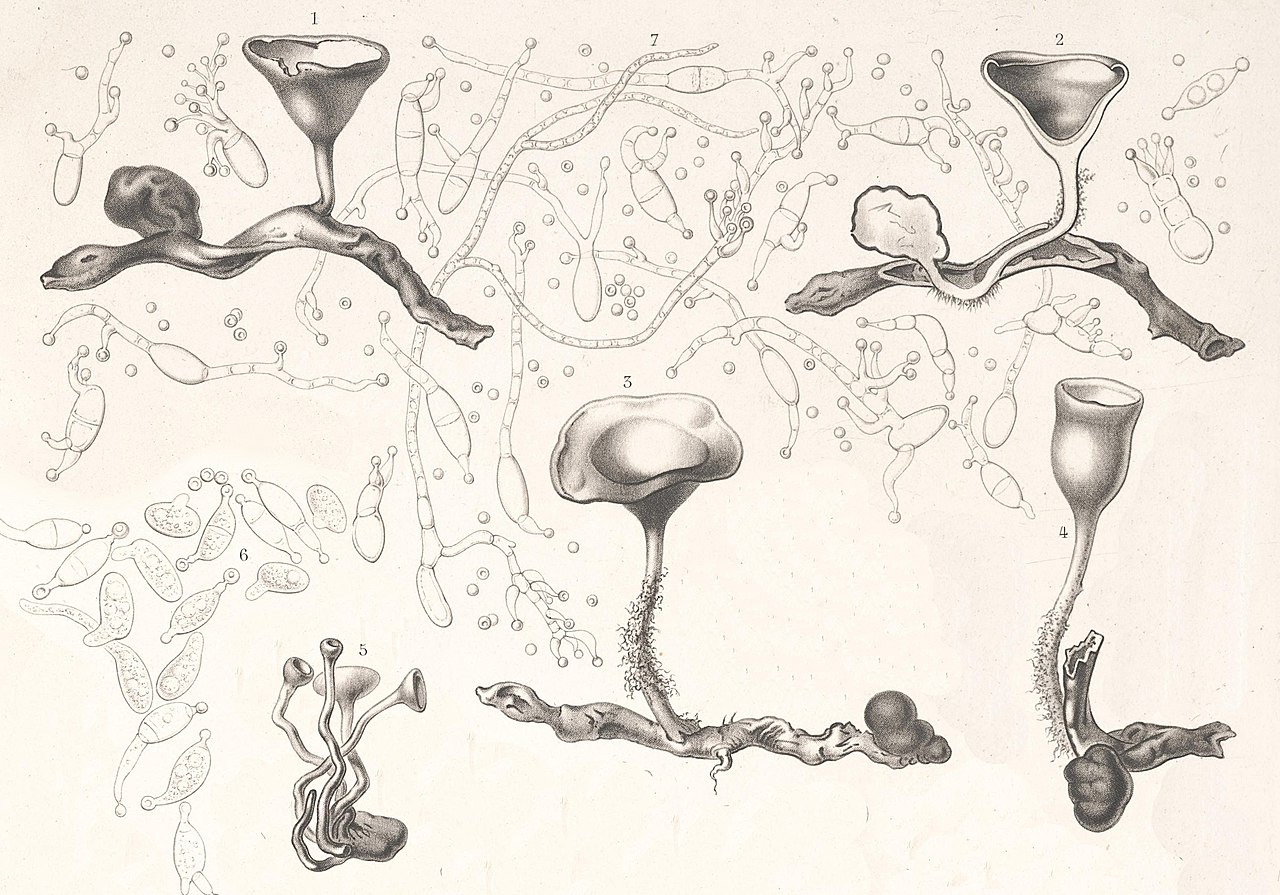
\includegraphics[width=\linewidth]{Figures/PezizaTuberosa.jpg}
%     \caption[Illustration of the fungus Dumontinia tuberosa.]{Illustration of the fungus Dumontinia tuberosa by physician, mycologist, and illustrator Charles Tulasne (1816–1884) in the book Selecta Fungorum Carpologia (1861–65). (Name of the original work: Peziza tuberosa parasite on Anemone nemorosa).}
%     \label{fig:figure-01}
% \end{figure}

% For the purpose of comparing or for other reasons, you can insert side-by-side figures using both the \verb|\begin{figure}| and \verb|\begin{subfigure}| environments. You can also refer to the sub-figure as \autoref{fig:figure-02.1} and \autoref{fig:figure-02.2}.

% \begin{figure}[!htpb]
%     \centering
%     \begin{subfigure}{0.45\textwidth}
%         \centering
%         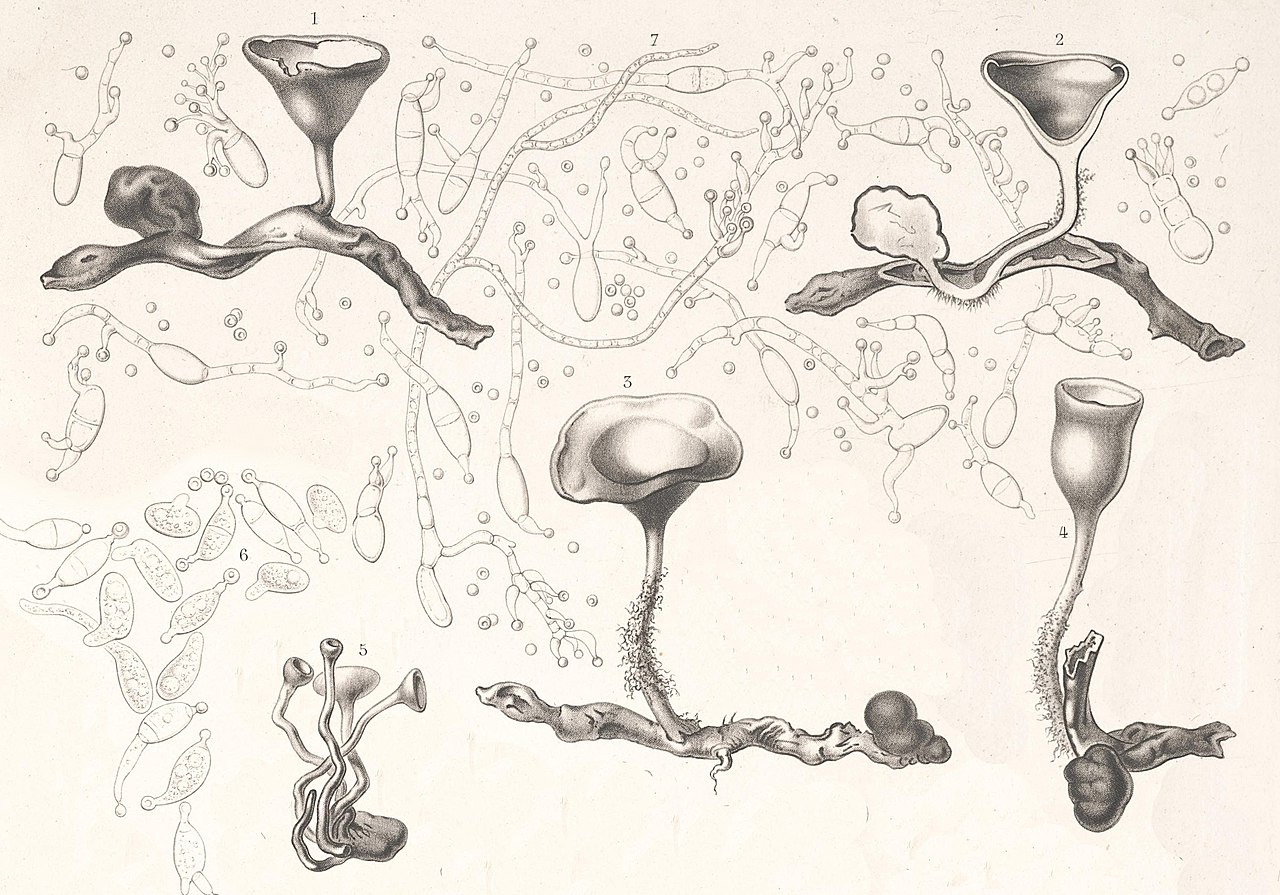
\includegraphics[width=0.9\textwidth]{Figures/PezizaTuberosa.jpg}
%         \caption{Caption for figure 1.}
%         \label{fig:figure-02.1}
%     \end{subfigure}
%     \hspace{.5cm} % Adjust the space as needed.
%     \begin{subfigure}{0.45\textwidth}
%         \centering
%         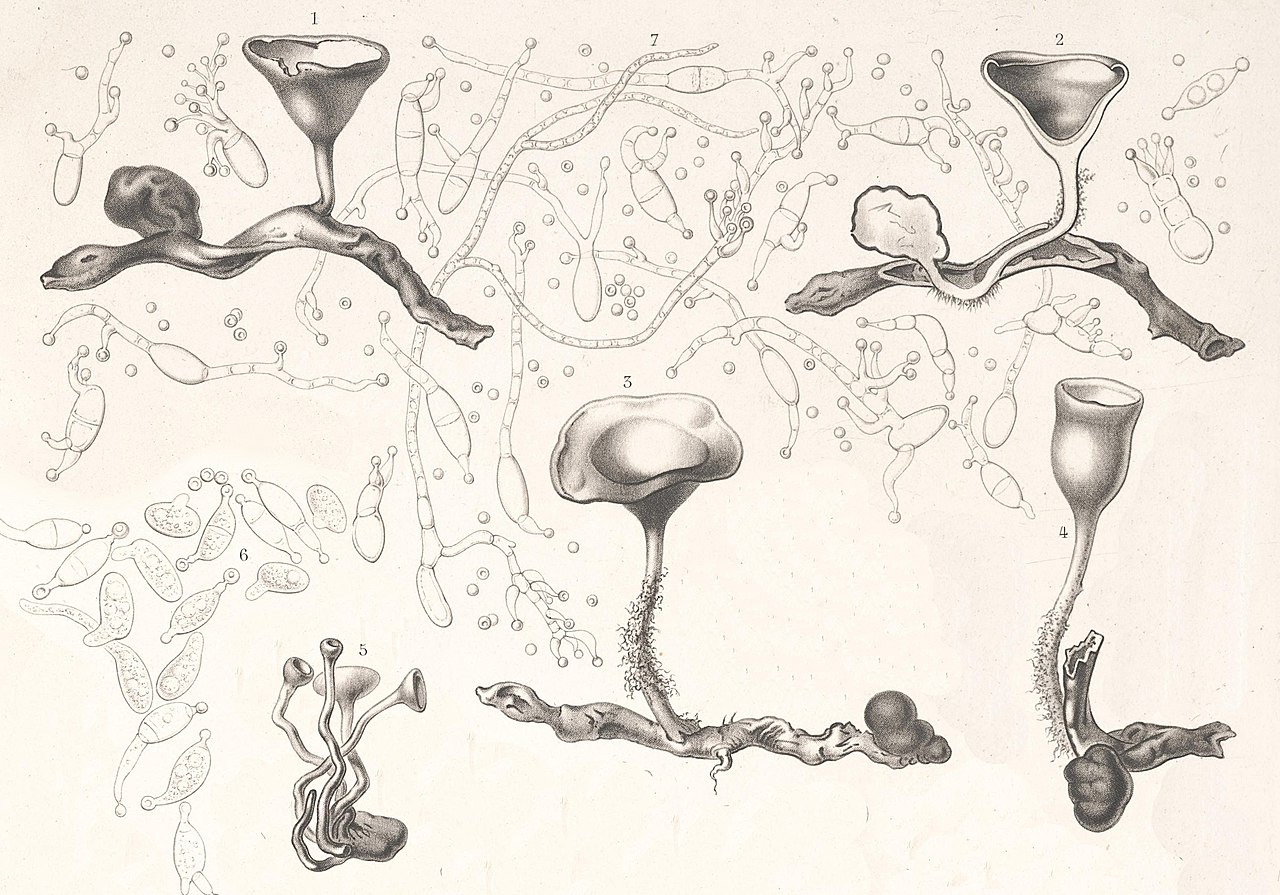
\includegraphics[width=0.9\textwidth]{Figures/PezizaTuberosa.jpg}
%         \caption{Caption for figure 2.}
%         \label{fig:figure-02.2}
%     \end{subfigure}
%     \caption{Overall caption of the figure.}
%     \label{fig:figure-02}
% \end{figure}

% \section{Tables}
% Tables are vital for presenting findings effectively. This chapter explores techniques for conveying information through tables using various template environments. Defining tables in \LaTeX\ seems complex, but this template simplifies the process.

% \begin{block}[tip]
% \textit{Prior to showcasing the different table environments, it's crucial to note that each one must be enclosed within a \texttt{\textbackslash begin\{table\}} environment. Additionally, it is recommended to utilise the \texttt{[!htpb]} float options for improved document placement. \textbf{This advice should be taken into consideration when positioning figures as well}.}
% \end{block}

% \subsection{Tabular Environment}
% The conventional \verb|\begin{tabular}| environment enables you to create a simple yet elegant table. \autoref{tab:table-01} is generated using a centering environment for added emphasis. It also incorporates the \verb|booktab| configuration for a more sophisticated table style.

% \begin{table}[!htpb]
%     \caption{A table showcasing the usage of the tabular environment.}
%     \label{tab:table-01}
%     \centering
%     \begin{tabular}{llc}
%         \toprule
%         \textbf{Header 01} & \textbf{Header 02} & \textbf{Header 03} \\ 
%         \midrule
%         Lorem Ipsum         & Pharetra Dolor    & $\checkmark$  \\
%         Amet Consectetuer   & Curabitur Aliquet & -             \\
%         Praesent Mauris     & Praesent Libero   & $\checkmark$  \\
%         \bottomrule
%     \end{tabular}
% \end{table}

% \subsection{Tabularx Environment}
% Employ the \verb|\begin{tabularx}| package to construct a table featuring automatically expanding multi-columns. To achieve this automatic behaviour for multi-columns, you can use the following environment: \verb|\begin{tabularx}{\textwidth}{lX}|, where \verb|X| is the column that will function as a multi-column. \autoref{tab:table-02} showcases the usage of the \verb|begin{tabularx}| environment.
% %Take note that we substitute \verb|X| in place of \verb|l| or \verb|c|, explicitly indicating that the column will function as a multi-column, occupying the entire available space.

% \begin{table}[!htpb]
%     \caption{A table showcasing the usage of the tabularx environment.}
%     \label{tab:table-02}
%     \begin{tabularx}{\textwidth}{lX}
%         \toprule
%         \textbf{Header 01} & \textbf{Header 02} \\ 
%         \midrule
%         Foo Bar Baz & Quisque cursus, metus vitae pharetra auctor, sem massa mattis sem, at interdum magna augue eget diam. \\
%         Ipsum Dolor & Vestibulum ante ipsum primis in faucibus orci luctus et ultrices posuere cubilia Curae; Curabitur aliquet quam id dui. \\
%         Dolor Sit & Phasellus condimentum elementum justo, quis interdum est sagittis ac. Vestibulum non arcu sit amet justo lobortis semper. \\
%         Amet Consectetuer & Integer nec odio praesent libero sed cursus ante dapibus diam sed nisi vestibulum non arcu. \\
%         Consectetuer Adipiscing & Nulla quis sem at nibh elementum imperdiet. Duis sagittis ipsum. Praesent mauris. \\
%         \bottomrule
%     \end{tabularx}
% \end{table}

% \subsection{Longtable Environment}
% At times, when dealing with exceptionally lengthy tables, it becomes necessary to split them across multiple pages. In \LaTeX, this can be achieved using the \verb|\begin{longtable}| environment. This environment is slightly more complex than others, as you need to define the header twice: once for the initial appearance of the table and again for when the table spans additional pages. This repeated header ensures the reader can correctly identify the columns on subsequent pages. Feel free to consult \autoref{tab:table-03} for a detailed demonstration of how the \verb|longtable| environment works.

% \begin{longtable}[c]{llll}
% \caption{A table showcasing the usage of the longtable environment.}
% \label{tab:table-03} \\
% \toprule
% \textbf{Names} & \textbf{E-Mails} & \textbf{Job/Role} \\ \midrule
% \endfirsthead
% %
% \multicolumn{4}{c}%
% {{\textit{\bfseries Table \thetable\ continued from previous page.}}} \\
% \toprule
% \textbf{Names} & \textbf{E-Mails} & \textbf{Job/Role} \\ \midrule
% \endhead
% %
% \bottomrule
% \addlinespace[1mm]
% \multicolumn{4}{r}%
% {{\textit{Continued on the next page.}}} \\
% \endfoot
% \bottomrule
% %
% \endlastfoot
% %
% Alice Johnson & alice.johnson@email.com & Project Manager \\
% Bob Thompson & bob.thompson@email.com & Data Analyst \\
% Charlie Davis & charlie.davis@email.com & Marketing Specialist \\
% David Miller & david.miller@email.com & QA Tester \\
% Emily White & emily.white@email.com & Graphic Designer \\
% Frank Martin & frank.martin@email.com & HR Coordinator \\
% Grace Turner & grace.turner@email.com & Financial Analyst \\
% Henry Lee & henry.lee@email.com & System Administrator \\
% Ivy Carter & ivy.carter@email.com & Customer Support \\
% Jack Wilson & jack.wilson@email.com & Frontend Developer \\
% Jane Reed & jane.reed@email.com & UX Designer \\
% Kevin Evans & kevin.evans@email.com & Product Manager \\
% Linda Adams & linda.adams@email.com & Accountant \\
% Mike Hill & mike.hill@email.com & Network Engineer \\
% Nina Garcia & nina.garcia@email.com & Business Analyst \\
% Oliver Smith & oliver.smith@email.com & Sales Representative \\
% Pamela Turner & pamela.turner@email.com & Legal Counsel \\
% Quincy Brown & quincy.brown@email.com & IT Consultant \\
% Rachel Moore & rachel.moore@email.com & Content Writer \\
% Samuel White & samuel.white@email.com & Research Scientist \\ 
% Amy Harris & amy.harris@email.com & Digital Strategist \\
% Brian Cook & brian.cook@email.com & Operations Manager \\
% Catherine Ross & catherine.ross@email.com & Brand Manager \\
% Daniel Green & daniel.green@email.com & Database Administrator \\
% Emma Taylor & emma.taylor@email.com & Social Media Manager \\
% Felix Carter & felix.carter@email.com & Compliance Officer \\
% Gloria Scott & gloria.scott@email.com & Procurement Specialist \\
% Harold Bennett & harold.bennett@email.com & DevOps Engineer \\
% Isla Cooper & isla.cooper@email.com & User Researcher \\
% James Black & james.black@email.com & Mobile App Developer \\
% Katie Brown & katie.brown@email.com & UI Designer \\
% Leo Perez & leo.perez@email.com & Scrum Master \\
% Megan Clark & megan.clark@email.com & Event Coordinator \\
% Nathan Ward & nathan.ward@email.com & Security Analyst \\
% Olivia Harris & olivia.harris@email.com & Corporate Trainer \\
% Paul King & paul.king@email.com & Territory Manager \\
% Queen Foster & queen.foster@email.com & Paralegal \\
% Rebecca Adams & rebecca.adams@email.com & Copy Editor \\
% Steven Martin & steven.martin@email.com & Robotics Engineer \\
% \end{longtable}

% \subsection{Complex Tables}
% Creating intricate tables in \LaTeX\ can be a somewhat challenging task. Therefore, we highly recommend using the \href{https://www.tablesgenerator.com/}{Table Generator}. With this tool, you can design your table with the desired style and then easily copy and paste it into your document. This approach simplifies the process and helps ensure the accurate representation of complex tables in your \LaTeX\ document. However, it's crucial to keep in mind that a table should be easily comprehensible for the reader and should not be overly complex. \textbf{The complexity of a table may impede understanding.} For example, \autoref{tab:table-04} presents a table with intricate details.

% \begin{table}[!htpb]
%     \caption{A table showcasing the usage of the complex tables.}
%     \label{tab:table-04}
%     \centering
%     \begin{tabular}{lcc}
%         \toprule
%         \multirow{2}{*}{\textbf{Component}} & \multicolumn{2}{c}{\textbf{Specifications}} \\
%         \cmidrule(lr){2-3}
%         & \textbf{Characteristic} & \textbf{Supported} \\
%         \midrule
%         \multirow{4}{*}{CPU} & Core Count (e.g., 8 Cores) & $\checkmark$ \\
%         & Clock Speed (e.g., 3.6 GHz) & $\checkmark$ \\
%         & Hyper-Threading & $\checkmark$ \\
%         & Integrated Graphics & - \\
%         \midrule
%         \multirow{4}{*}{GPU} & CUDA Cores (e.g., 5120) & $\checkmark$ \\
%         & Base Clock (e.g., 1.5 GHz) & $\checkmark$ \\
%         & Ray Tracing Support & $\checkmark$ \\
%         & Multi-GPU Support (SLI/CrossFire) & - \\
%         \midrule
%         \multirow{4}{*}{Memory} & Type (e.g., DDR5, GDDR6) & $\checkmark$ \\
%         & Capacity (e.g., 16 GB) & $\checkmark$ \\
%         & Memory Bandwidth (e.g., 448 GB/s) & $\checkmark$ \\
%         & ECC Support & - \\
%         \midrule
%         \multirow{3}{*}{Motherboard Features} & PCIe 5.0 Support & $\checkmark$ \\
%         & Wi-Fi 6E & $\checkmark$ \\
%         & Thunderbolt 4 & - \\
%         \bottomrule
%     \end{tabular}
% \end{table}

% \section{Lists}
% Creating lists in \LaTeX\ is straightforward, offering various options to suit your needs. You can generate a bullet list using \verb|\begin{itemize}|, or opt for a numbered list with \verb|\begin{enumerate}|. Below is an example with the \verb|\begin{itemize}| environment.

% \begin{itemize}
%   \item List entries start with the \verb|\item| command.
%   \item Individual entries are indicated with a black dot, a so-called bullet.
%   \item The text in the entries may be of any length.
% \end{itemize}

% As mentioned earlier, you can generate a numbered list using the \verb|\begin{enumerate}| environment. Here is an example:

% \begin{enumerate}
%   \item Items are numbered automatically.
%   \item The numbers start at 1 with each use of the \verb|enumerate| environment.
%   \item Another entry in the list.
% \end{enumerate}

% You can also nest list entries by creating a list inside another list of the same type. Here is an example:

% \begin{enumerate}
%     \item First level item
%     \item First level item
%     \begin{enumerate}
%         \item Second level item
%         \item Second level item
%     \begin{enumerate}
%         \item Third level item
%         \item Third level item
%     \end{enumerate}
%     \end{enumerate}
% \end{enumerate}

% \begin{block}[tip]
% \textit{Please note that the labels change automatically regardless of the environment being the same for every list. \textbf{This demonstrates that there's no need to worry about changing the environment for something different.}}
% \end{block}

% You can also modify the label of your list to something entirely different that suits your needs. To accomplish this, insert a new \verb|\item| and enclose your desired label in square brackets. For example, \verb|\item[!]| will result in an exclamation point as your new label. Below are some examples of modified labels.

% \begin{itemize}
%   \item This is my first point
%   \item Another point I want to make 
%   \item[!] A point to exclaim something!
%   \item[$\blacksquare$] Make the point fair and square.
%   \item[] A blank label?
% \end{itemize}

% Finally, you can create a description list. Unlike having a bullet point or a numbered label, a description list enables you to use custom descriptions that suit your list. In the example below, there are three \verb|\item| entries: one without a label, and two with descriptions.

% \begin{description}
%     \item[Item 1:] This is the first item with a description.
%     \item[Item 2:] Another item with a different description.
%     \item An item without a specific label.
% \end{description}

% \section{Code Listings}
% At times, you may want to include source code from your programs and applications within your document. To achieve this, you can use two nested environments: \verb|\begin{listing}| to create a listing with both caption and label, and \verb|\begin{minted}| for code highlighting. \autoref{listing:c-code} provides an example of a source code in C.

% \begin{listing}[!htpb]
% \caption{Hello world in C.}
% \label{listing:c-code}
% \begin{minted}{c}
% #include <stdio.h>
% int main() {
%    printf("Hello, World!"); /* printf() outputs the quoted string */
%    return 0;
% }
% \end{minted}
% \end{listing}

% The code mentioned above was inserted into the document. However, an alternative approach is to input your code from an external file. To do so, you just need to use the command \verb|\inputminted{CODE_LANGUAGE}{FILE}|. Of course, you should place that command inside of the \verb|\begin{listing}| environment. \autoref{listing:haskell-code} illustrates an example of Haskell source code that has been input from an external file.

% \begin{listing}[!htpb]
% \caption{Factorial in Haskell.}
% \label{listing:haskell-code}
% \inputminted{haskell}{Code/Factorial.hs}
% \end{listing}

% In some cases, when you simply want to highlight a specific command, it's recommended not to use \verb|listing| or \verb|minted|. Instead, you should utilise the \verb|\verb| command for inline highlighting or the \verb|\begin{verbatim}| environment for longer sections of highlighted code. An example of a lengthy \verb|verbatim| section is provided below, demonstrating how to create a \verb|listing| with an input code:

% \begin{verbatim}
% \begin{listing}[!htpb]
%     \inputminted{CODE_LANGUAGE}{FILE}
%     \caption{TEXT}
%     \label{TEXT}
% \end{listing}
% \end{verbatim}

% Sometimes it is necessary to display longer code that occupies more than one page. For this purpose, please use the environment \verb|\begin{longlisting}|. This environment will easily break your code into multiple pages for better readability without you worrying about the size of your code. An example is shown below in \autoref{listing:lisp-code}.

% \begin{longlisting}
% \caption{A sample of functions in Lisp.}
% \label{listing:lisp-code}
% \begin{minted}{lisp}
% (defun factorial (n)
%   "Calculate the factorial of a number."
%   (if (zerop n)
%       (* n (factorial (1- n)))))

% (defun fibonacci (n)
%   "Calculate the nth Fibonacci number."
%   (cond ((zerop n) 0)
%         ((= n 1) 1)
%         (t (+ (fibonacci (1- n)) (fibonacci (- n 2))))))

% (defun gcd (a b)
%   "Calculate the greatest common divisor of a and b."
%   (if (zerop b)
%       a
%       (gcd b (mod a b))))

% (defun primes-up-to (limit)
%   "Return a list of all prime numbers up to LIMIT."
%   (let ((primes '()))
%     (loop for i from 2 to limit
%           unless (some (lambda (p) (zerop (mod i p))) primes)
%           do (push i primes))
%     (nreverse primes)))

% (defun example-function (x)
%   "An example function to demonstrate Lisp capabilities."
%   (let ((result (list (factorial x)
%                       (fibonacci x)
%                       (gcd x 10)
%                       (primes-up-to x))))
%     (format t "Factorial of ~A: ~A~%" x (factorial x))
%     (format t "Fibonacci of ~A: ~A~%" x (fibonacci x))
%     (format t "GCD of ~A and 10: ~A~%" x (gcd x 10))
%     (format t "Primes up to ~A: ~A~%" x (primes-up-to x))
%     result))

% (example-function 10)
% \end{minted}
% \end{longlisting}

% \section{Equations}
% When writing equations and other mathematical expressions, \LaTeX~is a powerful and versatile tool. You can enter a formula in inline mode using the environment \verb|\(FORMULA\)| or use \verb|\begin{equation}| to display it in ``math mode'' with numbering. If you prefer not to display the equation number, you can use the environment \verb|\[FORMULA\]|.

% \vspace{.875em}
% \textbf{Example:} In physics, the mass-energy equivalence is expressed by the equation \(E=mc^2\), discovered in 1905 by Albert Einstein. In natural units ($c = 1$), the formula (\ref{eq:equation-01}) expresses the identity:

% \begin{equation}
% \label{eq:equation-01}
% E=m
% \end{equation}

% \textbf{Example:} Below is a equation -- \textit{without numbering} -- for the regularised loss function in supervised learning, combining the average prediction loss over the training dataset and an $L_2$ regularisation term to prevent overfitting:

% \[
% \mathcal{L}(\boldsymbol{\theta}) = \frac{1}{N} \sum_{i=1}^{N} \ell(y_i, f(\mathbf{x}_i; \boldsymbol{\theta})) + \lambda \|\boldsymbol{\theta}\|_2^2
% \]

% Equations can be a bit challenging to create, so we advise using an online editor, like the \href{https://latexeditor.lagrida.com/}{LaTeX Equation Editor}. Simply build your formulas there and copy and paste them into your document, either inline or in a math block, as shown above.

% \section{Footnotes}
% Sometimes it is important to present information that is not central to the main text in a footnote. In \LaTeX\, this can be easily achieved using the command \verb|\footnote{TEXT}|. The text will appear at the bottom of the page\footnote{This is a simple footnote.}.

% If you want to use footnotes within tables, it is best to reconsider, as \LaTeX\ does not provide an easy way to handle them. Instead, you can place a ``*'' wherever you want the footnote reference to appear. Then, below the table \textbf{but before ending the table environment}, place the ``*'' along with the footnote text. This will create a similar footnote, but it will appear below the table rather than at the bottom of the page.
% }

%%% Bibliography %%%
% \renewcommand{\refname}{Bibliography}
% \printbibliography[title={\refname},heading=bibintoc]

%%% Appendices: Work that *YOU* Developed %%%
\appendix
% \ifthenelse{\equal{\LanguageOption}{portuguese}}{
%     \addtocontents{toc}{\protect\contentsline{chapter}{Apêndices}{}{}}
% }{
%     \addtocontents{toc}{\protect\contentsline{chapter}{Appendices}{}{}}
% }

% % \ifthenelse{\equal{\MediaOption}{paper}}{\blankpage}{\clearpage}
% % \begin{center}
% %     \crimsonfont
% %     \thispagestyle{empty}
        
% %     \vspace*{\fill}
% %     \ifthenelse{\equal{\LanguageOption}{portuguese}}{%
% %         {\LARGE\fontsize{26}{26}\selectfont\textcolor{maincolor}{Apêndices}\par}
% %     }{%
% %         {\LARGE\fontsize{26}{26}\selectfont\textcolor{maincolor}{Appendices}\par}
% %     }
% %     \vspace*{\fill}
% % \end{center}
% \MediaOptionLogicBlank
% \chapter{Showcasing the First Appendix}
% \guideinfo{Appendices contain supplementary material \textbf{created by the author} that enhances the reader’s understanding of the dissertation while not being essential for following the primary narrative. These sections often include detailed tables, figures, complex calculations, or materials like survey questions and interview transcripts produced in the course of the research. The appendices allow readers to explore the research in greater detail, offering a deeper insight into methods and findings without interrupting the main body of work.}
% % Recommended dimensions for a landscape layout; adjust as needed.
% \begin{landscapemode}{297mm}{420mm}
%     \chapter{Showcasing the Second Appendix}
%     \blindtext[5]
% \end{landscapemode}

%%% Annexes: Work that *YOU DID NOT* Develop %%%
% \ifthenelse{\equal{\LanguageOption}{portuguese}}{
%     \addtocontents{toc}{\protect\contentsline{chapter}{Anexos}{}{}}
% }{
%     \addtocontents{toc}{\protect\contentsline{chapter}{Annexes}{}{}}
% }

% \setcounter{chapter}{11} % To start at the "L" chapter.
% \MediaOptionLogicAnnexes
% \begin{center}
%     \crimsonfont
%     \thispagestyle{empty}
        
%     \vspace*{\fill}
%     \ifthenelse{\equal{\LanguageOption}{portuguese}}{%
%         {\LARGE\fontsize{26}{26}\selectfont\textcolor{maincolor}{Anexos}\par}
%     }{%
%         {\LARGE\fontsize{26}{26}\selectfont\textcolor{maincolor}{Annexes}\par}
%     }
%     \vspace*{\fill}
% \end{center}
% \MediaOptionLogicBlank
% \chapter{Showcasing the First Annex}
% \guideinfo{Annexes are supplementary sections in a dissertation that provide additional information or external documents not essential to the main arguments but that support or complement the research. Unlike appendices, \textbf{annexes generally contain material that was not developed by the author}, such as reports, legal documents, or published datasets from external sources. This information is placed separately to keep the main content concise, allowing readers access to relevant external references without disrupting the dissertation's flow.}

%%% Back Page %%%
% \ifthenelse{\equal{\MediaOption}{paper}}{\blankpage}{}

% \clearpage
% \null
% \thispagestyle{empty}

% \ifthenelse{\equal{\CoverOption}{classic}}{
%     \newcommand\BackgroundPicBackPage{%
%     \put(0,0){%
%     \parbox[b][\paperheight]{\paperwidth}{%
%     \vfill
%     \centering
%     
\includegraphics[width=\paperwidth,height=\paperheight,keepaspectratio]{Figures/Theme/Back-Page-BG.pdf}%
%     \vfill
%     }}}
% }{
%     \newcommand\BackgroundPicBackPage{%
%     \put(0,0){%
%     \parbox[b][\paperheight]{\paperwidth}{%
%     \vfill
%     \centering
%     
\includegraphics[width=\paperwidth,height=\paperheight,keepaspectratio]{Figures/Theme/Back-Page-BG-W.pdf}%
%     \vfill
%     }}}
% }

% \AddToShipoutPictureBG*{\BackgroundPicBackPage}

% \newgeometry{margin=1.98cm, top=1.47cm, bottom=1.47cm}
% \noindent\clearpage
% \restoregeometry

\end{document}